\chapter{Continual Segmentation}
\label{chapter:segmentation}

\begin{chapabstract}
    In \acf{CIL}, new classes are learned with each new task. However, most of the literature in
    that domain focus on image classification where a single label is possible per sample. In
    \textbf{\acf{CSS}}, the setting is the same, but the implications are wildly different. In Semantic
    Segmentation, an image has one label per pixel. Therefore, an image could contain pixels from
    old, current, and future classes.
    \\
    In this chapter, I tackled the recent field of \acf{CSS}: I've first highlighted the main
    challenges of this domain: an important \textbf{catastrophic forgetting} linked to the higher complexity
    of segmentation images, and a \textbf{background shift} where images are partially labeled with
    only the current classes' ground-truth being present. Then, I've proposed multiple complementary
    methods across two papers to solve those challenges: I've designed an uncertainty-based
    hard pseudo-labeling loss, a multi-scale distillation loss inspired by my previous POD, and
    an efficient object rehearsal method.

    The work in this section has led to a publication to a conference paper (CVPR 2021) and a submission
    to a journal (TPAMI) still under review:

    \begin{itemize}
        \item \fullcite{douillard2020plop}
        \item \fullcite{douillard2021objectrehearsal}
    \end{itemize}

\end{chapabstract}
\newpage

\minitoc
\chapterwithfigures{\nameref*{chapter:segmentation}}
\chapterwithtables{\nameref*{chapter:segmentation}}

\ifthenelse{\boolean{skipSegm}}{\endinput}{}


\section{Introduction}
\label{sec:seg_intro}

Semantic segmentation aims to assign a label to each pixel of an image.
It allows the prediction of multiple objects in the same image, and moreover their exact position
and shape. This task recently flourished \citep{tao2020HRNet,zhang2020resnest,chen2018ZPSA} with
larger datasets with thousands of fully annotated images
\citep{zhou2017adedataset,neuhold2017mapillary}, increased computational power, and larger attention
\citep{wang2020axialdeeplab}. Unfortunately, the recent research in this area is often impracticable
for real-life applications: they mostly \textbf{need fully annotated data and require to be retrained from
    scratch if a new class is added to the dataset.} Ideally, one would wish to regularly expand a
dataset, only adding and labeling new classes and updating the model in accordance. This setup,
referred here as \textbf{\acf{CSS}}, has emerged very recently for specialized
applications
\citep{ozdemir2018learnthenewkeeptheold,ozdemir2019segmentationanotomical,tasar19incrementsegmentationremotesensing}
before being proposed for general segmentation datasets
\citep{michieli2019ilt,cermelli2020modelingthebackground}.


In particular, in this chapter, we argue that two problems arise when performing \ac{CSS} with
\acs{DCNN}. The first one, inherited from continual learning, is \textbf{catastrophic
    forgetting}~\citep{robins1995catastrophicforgetting}, already well detailed in the previous chapters
including \autoref{chapter:related}. One of the most efficient methods to avoid forgetting is rehearsal
learning (\autoref{sec:related_rehearsal}) where we store a few images from previous tasks.
Unfortunately, this solution has difficulty in the context of segmentation where multiple classes
can be in the same image, and where the storage cost is high and images are partially labeled. The
second challenge, specific to \ac{CSS}, is the semantic shift of the background class. In a
traditional semantic segmentation setup, all object categories are predefined, and the "background"
class contains pixels that do not belong to any of these classes. However, in \ac{CSS}, the
background contains pixels that do not belong to any of the \textit{current} classes. Thus, for a
specific learning step, the background can contain both future classes, not yet seen by the model,
as well as old classes. Thus, if nothing is done to distinguish pixels belonging to the real
background class from old class pixels, this \textbf{background shift} phenomenon risks exacerbating
the catastrophic forgetting even further \citep{cermelli2020modelingthebackground}. This issue also
has an impact on the selection of the old data we want to store. Because some currently learned
classes are annotated as background in the old data, this may degrade the performance of these
classes if one naively treat them as background to fine-tune the current model.

We tackle the first challenge of catastrophic forgetting by designing a constraint enforcing a
similar behavior between the old and current model. Specifically, we leverage intermediary
representations of the convolutional networks to ensure that similar patterns are extracted through
time. \textbf{This feature-based constraints, called Local POD, fully exploits the global and local
    scale necessary to semantic segmentation through a multi-scale design}. The second challenge,
background shift, is greatly alleviated \textbf{a confidence-based pseudo-labeling strategy to
    retrieve old class pixels within the background}. For instance, if a current ground truth mask only
distinguishes pixels from class \texttt{sofa} and background, our approach allows assigning old
classes to background pixels, e.g. classes \texttt{person}, \texttt{dog} or \texttt{background} (the
semantic class). We name PLOP the model exploiting those two contributions. We then propose
\textbf{an extension called PLOPLong that aims to excel on long continual learning scenarios}. This
new model exploits cosine normalization to adapt the classifier and the Local POD resulting in an
improving robustness to the discrepancy between old and new classes. Moreover, PLOPLong features a
modified batch normalization which reduces the sensitivity of the model to moving statistics seen
across tasks in continual learning. Finally, we are the first to investigate rehearsal learning in
the frame of \ac{CSS}. We propose a baseline approach that is based upon rehearsing complete images.
However, in practice, this seemingly classic rehearsal is not as trivial in our context as the
labeling is partial: hence, once again, we need to complete the rehearsed images after each step by
filling the background with the missing old classes. While significantly improving performances, we
show that such approach has two main drawbacks. First, it is memory intensive, as the whole images
shall be rehearsed at each \ac{CSS} step. Second, despite the large number of pixels in the images,
we argue that the images contain few, sparse useful information. Consequently, we design \textbf{a
    novel rehearsal method, that we named ``Object Rehearsal``, that consists in selecting only
    non-regular objects-centered patches as candidates for rehearsal}. Those objects, belonging to old
classes, are combined into the images of new classes \textit{via} careful image editing. We
empirically show that this new rehearsal method surpasses classic rehearsal with pseudo-labeling,
while being up to 146x times more memory efficient.

From a practical point of view, our proposed methods (PLOP, PLOPLong, and Object Rehearsal) showed
three important results. First, we achieve the state-of-the-art performance on several challenging
datasets. Secondly, we propose several novel scenarios to further quantify the performances of \ac{CSS}
methods when it comes to long term learning, class presentation order and domain shift. Last but not
least, we show that our model contributions largely outperform every \ac{CSS} approach in these
scenarios.

To sum it up, our contributions are four-folds:
\begin{itemize}
    \item We propose a multi-scale spatial distillation loss to better retain knowledge through the
          continual learning steps, by preserving long- and short-range spatial statistics, avoiding
          catastrophic forgetting.
    \item We introduce a confidence-based pseudo-labeling strategy to identify old classes for the
          current background pixels and deal with background shift.
    \item We propose PLOPLong, a carefully designed refinement of our method for dealing with long
          \ac{CSS} scenarios. The extension comes from an adaptation of PLOP's classifier and Local POD
          distillation as well as batch re-normalization for better handling of both catastrophic
          forgetting and background shift, respectively.
    \item We design a novel memory-efficient Object rehearsal learning procedure that consists in
          storing and carefully pasting objects through selective erasing of foreground objects. It
          results in better performance for a fraction of the memory cost imposed by classic
          rehearsal.
\end{itemize}

Additionally, We show that our PLOP significantly outperforms state-of-the-art approaches in existing
scenarios and datasets for \ac{CSS}, as well as in several newly proposed challenging benchmarks on new
datasets. Furthermore, we show that PLOPLong leads to superior performances on longer \ac{CSS} scenarios.
Last but not least, we show that performance of \ac{CSS} models can be greatly improved where rehearsal
learning is an option. In such cases, the proposed Object rehearsal allows reaching high accuracies
with low memory footprint.

\section{Related Work}
\label{sec:seg_related}

Continual Semantic Segmentation is a relatively young field that started getting traction following
\cite{michieli2019ilt,cermelli2020modelingthebackground}. However, this field is at the intersection
of many popular topics. Therefore, we start this section with an overview of recent advances in
segmentation. We then follow with a more in-depth discussion of existing approaches to \ac{CSS}. For
a thorough discussion of Continual Learning, please refer to \autoref{chapter:related}.

\paragraph{Semantic Segmentation} methods based on Fully Convolutional Networks (FCN)
\citep{long2015fcn,sermanet2014overfeat} have achieved impressive results on several segmentation
benchmarks ~\citep{everingham2015pascalvoc,
    cordts2016cityscapes,zhou2017adedataset,caesar2018cocoostuff}. These methods improve the
segmentation accuracy by incorporating more spatial information or exploiting contextual information
specifically. Atrous convolution~\citep{chen2018deeplab,mehta2018espnet} and encoder-decoder
architecture~\citep{ronneberger2015UNet,noh2015deconvolution,badrinarayanan2017segnet} are the most
common methods for retaining spatial information. Examples of recent works exploiting contextual
information include attention
mechanisms~\citep{yuan2018ocnet,zhao2018psanet,fu2019DANet,huang2019CCNet,yuan2020ocr,tao2020HRNet,zhang2020resnest},
and fixed-scale aggregation
~\citep{zhao2017PSPNet,chen2018deeplab,chen2018ZPSA,zhang2018ContextEncoding}.

\paragraph{Continual Semantic segmentation}: Despite enormous progress in the two
aforementioned areas respectively, segmentation algorithms are mostly used in an offline setting,
while continual learning methods generally focus on image classification. Recent works extend
existing continual learning methods \citep{li2018lwf,hou2019ucir} for specialized applications
\citep{ozdemir2018learnthenewkeeptheold,ozdemir2019segmentationanotomical,tasar19incrementsegmentationremotesensing}
and general semantic segmentation \citep{michieli2019ilt}. The latter considers that the previously
learned categories are properly annotated in the images of the new dataset. This is an unrealistic
assumption that fails to consider the background shift: pixels labeled as background at the current
step are semantically ambiguous, in that they can contain pixels from old classes (including the
real semantic background class, which is generally deciphered first) as well as pixels from future
classes. \cite{cermelli2020modelingthebackground} propose a novel classification and
distillation losses. Both handle the background shift by summing respectively the old logits with
the background logits and the new logits with the background. We argue that a distillation loss
applied to the model output is not strong enough for catastrophic forgetting in \ac{CSS}. Furthermore,
their classification loss doesn't preserve enough discriminative power w.r.t the old classes when
learning new classes under background shift. We introduce our PLOP framework that solves more
effectively those two aspects. \cite{yu2020continualsegmentationselftraining} proposed to
exploit an external unlabeled dataset in order to do self-training with a pseudo-labeling loss; we
show that our model while not designed with this assumption in mind can outperform their
performance. \cite{cermelli2020fewshotcontinualsegm} creates a novel setting of
continual \textit{few-shots} segmentation, we implement their method in our setting and draw
inspiration from it to further improve PLOP. \cite{michieli2021sdr} draws
inspiration from the metric learning literature to conceive a model for continual segmentation that
exploits prototypes updated with an exponential moving average of the mean batch features.

\paragraph{Positioning:} Contrary to previous works in continual segmentation
\citep{michieli2019ilt,cermelli2020modelingthebackground} which reduced slightly forgetting through
distillation of the probabilities, we propose a stronger constraint based on global and local
statistics extracted from intermediary features. Moreover, background shift is often not considered
\citep{michieli2019ilt} or only weakly tackled \citep{cermelli2020modelingthebackground}, while we
propose to eliminate it through segmentation maps completion with pseudo-labeling. Finally, none of
the work proposed rehearsal methods for \ac{CSS}, while we propose a non-trivial method based on image
rehearsal and further improve it with a more data-efficient method based with object rehearsal.


\section{PLOP and PLOPLong models}
\label{sec:seg_plop}

\begin{figure}
    \centering
    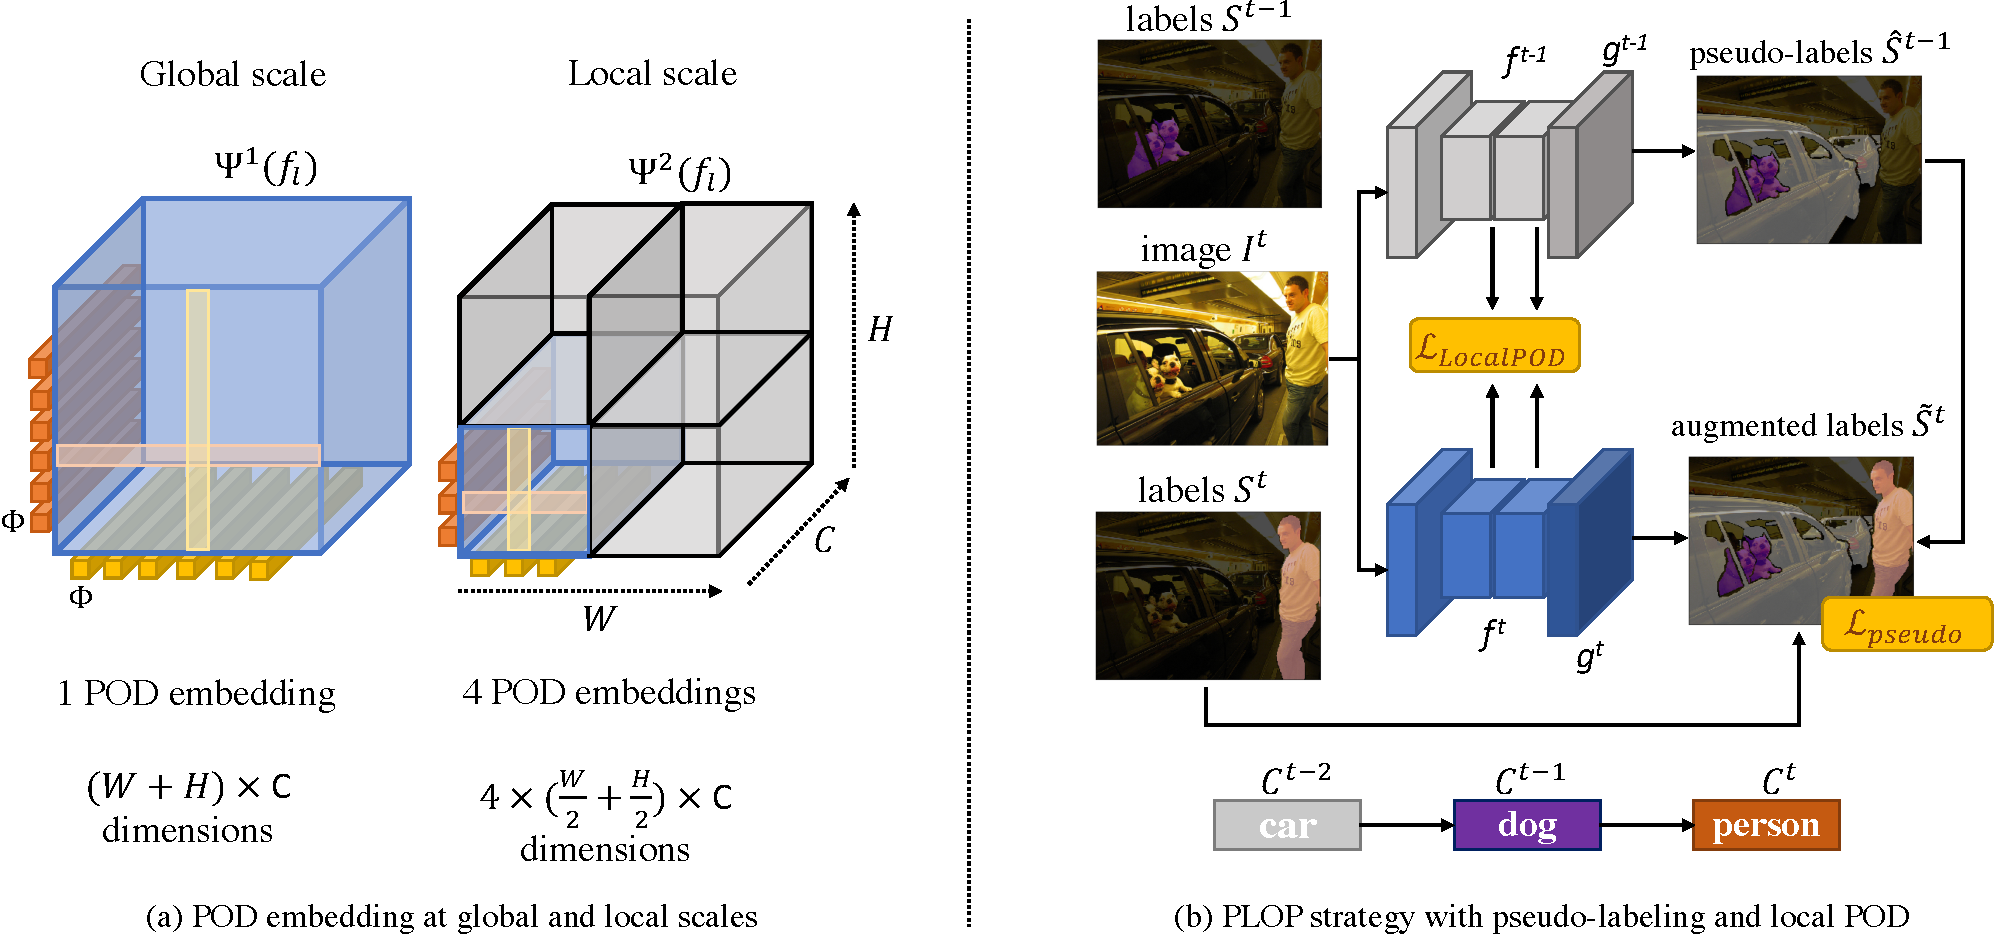
\includegraphics[width=\linewidth]{images/seg/plop_strategy.pdf}
    \caption{Local POD details and the complete PLOP strategy. (a) Local POD consists in POD
        embeddings compute at multiple scale. The global scale aggregates statistics across the
        whole features maps while the local scale focuses on finer details.  (b) The model
        incrementally learns new classes (\textit{e.g.} \texttt{car}, \texttt{dog},
        \texttt{person}). Only the current class (\texttt{person}) is labeled while previous classes
        are folded into the background. We use the previous model $g^{t-1} \circ f^{t-1}$ to
        generate pseudo-labels $\hat{\mcS}^{t-1}$ regarding the old classes to alleviate this
        ambiguity, and complete the labels $\mcS^t$ which are then used as ground-truth in
        $\mcL_\text{pseudo}$. The Local POD distillation is applied at multiple levels of the
        features extractors $f^{t-1}$ and $f^t$.}
    \label{fig:seg_model_plop}
\end{figure}

The model description is organized as follows: we first detail the continual protocol and the
notations. Then, we tackle the issue of catastrophic forgetting by designing an adapted distillation
loss, and we alleviate the background shift by proposing an uncertainty-based pseudo-labeling. Drawing
ideas from the continual learning literature, we propose an extension of PLOP specialized for
long-range continual training that we nickname PLOPLong. Finally, we detail the limits of rehearsal
learning in segmentation, propose a naive adaptation to the problem, and then deliver our carefully
designed method.

\subsection{Framework and notations}\label{sec:seg_overview}

For most of the notations, please refer to \autoref{tab:related_notation}. The slight difference in
this chapter, is that instead of working on pair of classification image with a single label $(\vx,
    y)$, we'll work on pairs of image and segmentation maps where each pixel has a class $(\mcI^t,
    \mcS^t)$. Here, the task identifier $t$ is even more important because the segmentation maps $\mcS$,
for a same image, will evolve through the tasks. Indeed, in the considered benchmarks (detailed
later in \autoref{sec:seg_exp}), an image is only labeled for the current classes $\mcS^t$. The
previous $\mcC^{1:t-1}$ or future classes $\mcC^{t+1:T}$ the image may contain are not labeled, and
considered as the special class ``\textit{background}''. However, at test-time, a model at step $t$
must be able to discriminate between all the classes that have been seen so far, \textit{i.e.}
$\mcC^{1:t}$.

This leads us to identify two major pitfalls in \ac{CSS}: the first one, inherited from continual
learning, is catastrophic forgetting \cite{robins1995catastrophicforgetting}. It suggests that a
network will completely forget the old classes $\mcC^{1:t-1}$ when learning the new ones $\mcC^t$.

Furthermore, catastrophic forgetting is aggravated by the second pitfall, specific to \ac{CSS}, that
we call background shift: at step $t$, the pixels labeled as background are indeed ambiguous, as
they may contain either old (including the real background class, predicted in $\mcC^{1}$) or future
classes.

We define our model at step $t$ as a composition of a feature extractor $f^t(\cdot)$ (a ResNet 101
\cite{he2016resnet} backbone and a classifier $g^t(\cdot)$. The output predicted segmentation map
can then be written $\hat{\mcS}^t = g^t \circ f^t(\mcI)$. We denote the intermediate features at
each layer of the feature extractor $f_l^t(\cdot)\,,\, l \in \{1, \dots L\}$. Finally, we denote the
set of learnable parameters of $f^t$ and $g^t$ as $\Theta^t$.


\subsection{Overcoming catastrophic forgetting in CSS with local
    distillation}\label{sec:seg_distillation}

In this section, we propose to tackle the issue of catastrophic forgetting in continual learning in
general and in \ac{CSS} in particular. An effective method for doing so involves setting constraints
between the old ($g^{t-1} \circ f^{t-1}$) and current ($g^{t} \circ f^{t}$) models. These
constraints aim at enforcing a similar behavior between both models and in turn reduce the loss of
performance on old classes. A common such constraint is based on applying knowledge distillation
\cite{hinton2015knowledge_distillation,li2018lwf} between the predicted probabilities of both
models. When applied to \ac{CSS}, such distillation loss must be carefully balanced to find a good
trade-off between rigidity (\textit{i.e.} too strong constraints, resulting in not being able to
learn new classes) and plasticity (\textit{i.e.} enforcing loose constraints, which can lead to
catastrophic forgetting of the old classes).

In \autoref{chapter:regularization}, more precisely in \autoref{sec:podnet}, we designed POD, short
for Pooled Output Distillation. Rather than solely constraining the output model probabilities, POD
enforces consistently between intermediary statistics of both models. In practice, for a feature map
$\vx$, we define a POD embedding $\Phi(\cdot)$ as:
%
\begin{equation}
    \Phi(\vx) = \left[\frac{1}{W} \sum_{w=1}^W \vx[:,w,:] \bigg\Vert \frac{1}{H} \sum_{h=1}^H \vx[h,:,:]\right] \in \mathbb{R}^{(H + W) \times C}\,,
    \label{eq:seg_pod_embedding}
\end{equation}
%
where $[\cdot\,\|\,\cdot]$ denotes concatenation over the channel axis. The POD embedding is thus
computed as the concatenation of the $H \times C$ width-pooled slices and the $W \times C$
height-pooled slices of $\vx$ and captures long-range statistics across the whole features maps. The
POD distillation loss then consists in minimizing the $\mathcal{L}_2$ distance between POD
embeddings computed at several layers $l \in \{1, \dots, L\}$, w.r.t the current model parameters
$\Theta^t$:
%
\begin{equation}
    \mcL_\text{pod}(\Theta^t) = \frac{1}{L} \sum_{l = 1}^L \left\Vert  \Phi(f^t_l(\mcI)) -  \Phi(f^{t-1}_l(\mcI)) \right\Vert^2\,.
    \label{eq:seg_pod_loss}
\end{equation}
%
POD yielded state-of-the-art results in continual learning for image classification, especially when
large numbers of tasks are considered, a case where the aforementioned plasticity-rigidity trade-off
becomes even more crucial. Another interest arises in the context of \ac{CSS}: the long-range statistics
computed across an entire axis (horizontal or vertical) which reminds recent work on attention for
segmentation \citep{wang2020axialdeeplab,huang2020ccnet,park2020csc} which aim to enlarge the
receptive field through global attention/statistics \citep{wang2020axialdeeplab}. In the frame of
classification, it is, to a certain extent, necessary to discard spatial information through global
pooling. However, conversely, semantic segmentation requires preservation of both long-range and
short-range statistics, making a distillation loss such as POD suboptimal for that purpose.


Following this reflection, and inspired by the multi-scale literature
\citep{lazbnik2006spatial_pyramid_matching,he2014spatialpyramidpooling}, we design a distillation
loss, called Local POD that retain the long-range spatial statistics while also preserving the local
information. The proposed Local POD consists in computing the width and height statistics at
different scales $\{1/2^s\}_{s=0 \dots S}$, as illustrated in \autoref{fig:seg_model_plop} (a). At a
given level $l$ of the feature extractor, $s^2$ POD embeddings are computed per scale $s$ and
concatenated:
%
\begin{equation}
    \Psi^s(\vx) = \left[ \Phi(\vx^s_{0,0}) \| \dots \| \Phi(\vx^s_{s-1,s-1}) \right] \in \mathbb{R}^{S \times (H + W) \times C}\,,
    \label{eq:seg_localpod_embedding1}
\end{equation}
%
where $\forall i = 0 \dots s-1$, $\forall j = 0 \dots s-1$, $\vx^s_{i,j} = \vx[i H/s:(i+1) H/s, j
        W/s:(j+1) W/s,:]$ is a sub-region of the embedding tensor $\vx$ of size $W/s \times H/s$. We
then concatenate (along the channel axis) the Local POD embeddings $\Psi^s(\vx)$ of each
scale $s$ to form the final embedding:
%
\begin{equation}
    \Psi(\vx) = \left[ \Psi^1(\vx) \| \dots \| \Psi^S(\vx) \right] \in \mathbb{R}^{(1 + \dots + S) \times (H + W) \times C}\,.
    \label{eq:seg_local_pod}
\end{equation}
%
Similarly to POD, we compute Local POD embeddings for every layer $l \in \{1, \dots, L\}$ of both
the old and current models. The resulting loss is thus:
%
\begin{equation}
    \mcL_{\scriptstyle\text{LocalPod}}(\Theta^t) = \frac{1}{L} \sum_{l = 1}^L \left\Vert  {\Psi}(f^t_l(I)) -  {\Psi}(f^{t-1}_l(I)) \right\Vert^2\,.
    \label{eq:seg_local_pod_loss}
\end{equation}
%
Thus, notice that the first scale of Local POD ($1/2^0$) is similar to the original POD and models
long-range dependencies across the entire image. The subsequent scales ($s=1/2^1, 1/2^2 \dots$),
enforce short-range dependencies. Thus, the proposed Local POD tackles the problem of catastrophic
forgetting by modeling and preserving long and short-range statistics between the old and current
models, throughout the \ac{CSS} steps.


\subsection{Pseudo-labeling to fix background shift}\label{sec:seg_hardpl}

In addition to catastrophic forgetting, a successful \ac{CSS} approach shall handle the background shift
problem, thus shall take into account the ambiguity of pixels labelled as background at each step.
We propose a pseudo-labeling strategy that ``\textit{completes}'' the ambiguous background labels.
Pseudo-labeling \citep{lee2013pseudolabel} is commonly used in domain adaption for semantic
segmentation
\citep{vu2019advent,li2019bidirectionallearning,zou2018classbalancedselftraining,saporta2020esl}
where a model is trained to match both the labels of a source dataset and the pseudo-labels (usually
obtained using the same predictive model, in a self-training fashion) of an unlabeled target
dataset. In this case, the knowledge acquired on the source dataset helps the model to generate
labels for the target dataset. In the frame of \ac{CSS}, at each step, we use the predictions of the old
model to decipher previously seen classes among the ambiguous background pixels, as illustrated in
\autoref{fig:seg_model_plop}. The pseudo-labeling rely on the previous model which can be uncertain
for some pixels due to inherent bias to the optimization and because of the forgetting. Therefore,
in order to avoid propagate errors through incorrect pseudo-labels, we filter out the most uncertain
ones based on an adaptive entropy-based threshold.

Formally, let $\mcN^t=\operatorname{card}(\mcC^{t})-1$ the cardinality of the current classes
excluding the background class. Let $\hat{\mcS}^{t} \in \mathbb{R}^{W,H,1+\mcN^1 +\dots + \mcN^t}$
denotes the predictions of the current model (which includes the real background class, all the old
classes as well as the current ones). We define $\tilde{\mcS}^{t} \in \mathbb{R}^{W,H,1+\mcN^1
        +\dots + \mcN^t}$ the target as step $t$, computed using the one-hot ground-truth segmentation map
$\mcS^{t} \in \mathbb{N}^{W,H,1+\mcN^t}$ at step $t$ as well as pseudo-labels extracted using the
old model predictions $\hat{\mcS}^{t-1} \in \mathbb{R}^{W,H,1+\mcN^1 +\dots + \mcN^{t-1}}$ as
follows:
%
\begin{equation}
    \footnotesize
    \tilde \mcS^{t}\left(w,h,c\right)= \mkern-5mu \left\{\begin{array}{ll}
        \mkern-10mu 1 \mkern-27mu & \text { if } S^{t} (w,h,c_{bg})=0 \text { and } c = \argmax \limits_{c' \in \mcC^{t}} \mcS^{t}(w,h,c')                                     \\
        \mkern-10mu 1 \mkern-27mu & \text { if } \mcS^{t}(w,h,c_{bg})=1 \text { and } c = \mkern-8mu \argmax \limits_{c' \in \mcC^{1:t-1}} \mkern-6mu \hat{\mcS}^{t-1}(w,h,c') \\
        \mkern-10mu 0 \mkern-27mu & \text { otherwise }                                                                                                                        \\
    \end{array}\right.
    \label{eq:seg_pseudo_bis}
\end{equation}
%
In other words, in the case of non-background pixels we simply copy the ground truth label.
Otherwise, we use the class predicted by the old model $g^{t-1}(f^{t-1}(\cdot))$. This pseudo-label
strategy allows to assign each pixel labelled as background his real semantic label if this pixel
belongs to any of the old classes. However, pseudo-labeling all background pixels can be
unproductive, e.g. on uncertain pixels where the old model is likely to fail. Therefore, we only keep
pseudo-labels where the old model is deemed ``\textit{confident}'' enough.
\autoref{eq:seg_pseudo_bis} is modified to take into account this uncertainty:
%
\begin{equation}
    \scriptsize
    \tilde \mcS^{t}\left(w,h,c\right)\mkern-5mu = \mkern-5mu \left\{\begin{array}{ll}
        \mkern-14mu 1 \mkern-27mu & \mkern-8mu \text { if } \mcS^{t} \mkern-4mu (w,h,c_{bg})\mkern-4mu = \mkern-4mu 0 \text { and } c \mkern-4mu = \mkern-4mu \argmax \limits_{c' \in \mathcal{C}^{t}} \mcS^{t} \mkern-4mu (w,h,c')                                                                         \\
        \mkern-14mu 1 \mkern-27mu & \mkern-8mu \text { if } \mcS^{t} \mkern-4mu (w,h,c_{bg}) \mkern-4mu = \mkern-4mu 1 \text { and } c \mkern-4mu = \mkern-12mu \argmax \limits_{c' \in \mathcal{C}^{1:t-1}} \mkern-6mu \hat \mcS^{t-1} \mkern-4mu (w,h,c') \text{ and } u \mkern-4mu < \mkern-4mu \tau_{c} \\
        \mkern-14mu 0 \mkern-27mu & \mkern-4mu \,\text { otherwise\,, }                                                                                                                                                                                                                                     \\
    \end{array}\right.
    \label{eq:seg_pseudo_bis_uncertain}
\end{equation}
%
By notation abuse, $u$ is function $u(\mcS^t(w, h))$ that measures the uncertainty of the current
model given a pixel $\mcI(w,h)$. $\tau_{c}$ denotes a class-specific uncertainty threshold. Hence,
in the case where the old model is uncertain ($u \ge \tau_c$) about some pixels, they will be
ignored in the final classification loss. Our framework is agnostic to the type of uncertainty used,
but in practice we define it as the entropy. Therefore, we use for $u$ the current model's per-pixel
entropy $u(\mcS^t(w, h)) = -\sum_{c \in C^{1:t}} \mcS^t(w, h, c) \log \mcS^t(w, h, c)$. Likewise,
the class-specific threshold $\tau_c$ is computed from the median entropy of the old model over all
pixels of $\mcD^t$ predicted the class $c$ for all $c \in \mcC^{1:t-1}$ as proposed by
\cite{saporta2020esl}. Consequently, the cross-entropy loss with pseudo-labeling of the old classes
can be written as:
%
\begin{equation}
    \mcL_\text{pseudo}(\Theta^t)=- \frac{\nu}{WH} \sum_{w,h}^{W,H} \sum_{c \in \mathcal{C}^{t}} \tilde \mcS\left(w,h,c\right) \log \hat \mcS^{t}\left(w,h,c\right)\,.
    \label{eq:seg_pseudo_loss}
\end{equation}
%
We reduce the normalization factor $WH$ by as much discarded pixels. To avoid giving disproportional
importance to the pixels belonging to new classes (which aren't discarded), we introduce in
\autoref{eq:seg_pseudo_loss} an adaptive factor $\nu$, which is the ratio of accepted old classes
pixels over the total number of such pixels. \textit{i.e.} if most of the image is uncertain, the
overall importance of the image relative to other images in the batch is reduced. The overall
behavior of our pseudo-labeling is illustrated in \autoref{fig:seg_model_plop}.

We call our final model PLOP (standing for Pseudo-labeling and LOcal Pod). PLOP's final loss is a
weighted combination of \autoref{eq:seg_local_pod_loss} and \autoref{eq:seg_pseudo_loss}:
%
\begin{equation}
    \mcL(\Theta^t) = \underbrace{\strut \mcL_\text{pseudo}(\Theta^t)}_\text{classification} + \lambda\underbrace{\strut \mcL_\text{localPod}(\Theta^t)}_\text{distillation}\,,
    \label{eq:seg_complete_loss}
\end{equation}
%
\noindent with $\lambda$ a hyperparameter. PLOP, while already very competitive, can face difficulties when
dealing with long continual settings, \textit{i.e.} for which the number of steps grows larger. For
this reason, we propose PLOPLong, an extension of PLOP for dealing with such cases.

\subsection{PLOPLong: a specialization for long settings}\label{sec:seg_plopv2}

While the proposed method already achieves satisfying results in traditional \ac{CSS} scenarios, it might
struggle to deal with longer settings due to two major drawbacks, namely specialization of the
classifier towards recent classes, and the shifts of the batch normalization layers.

First, we observe that in \ac{CSS} the classifier weights tend to be specialized for the last classes to
the detriment of older classes \citep{hou2019ucir}. Several solutions exist that aim at correcting
this bias
\citep{wu2019bias_correction,belouadah2019il2m,zhao2020weightalignement,luo2018cosine_classifier}, and
we choose the cosine normalization. In practice, we replace the classifier by a cosine classifier
\citep{luo2018cosine_classifier}, where the final inner product is discarded in favor of a cosine
similarity. By doing so, all class weights --both old and new-- have a constant magnitude of 1,
which drastically reduces the bias towards new classes. The classifier $g^t$ is in segmentation a
pointwise ($1\times1$ kernel) convolution which doesn't alter the spatial organization but maps the
$ch$ features channels to $\mcC^{1:t}$ channels, one per class to predict. This pointwise
convolution can be seen as a fully-connected layer that is applied independently to each pixel.
Therefore, the classifier $g^t$ has $\{\theta_c^t \in \mathbb{R}^{ch} | \forall c \in \mcC^{1:t}\}$.
The cosine normalization can then be express as:
%
\begin{equation}
    \hat{\mcS}(w, h, c) = \frac{\alpha \langle \theta^t_c, \vh(w, h) \rangle}{\Vert \theta^t_c \Vert^2 \Vert \vh(w, h) \Vert^2}\,
    \label{eq:seg_cosine_classifier}
\end{equation}
%
\noindent with $\alpha$ a learned scalar parameter initialized to 1 and helping the convergence, and $\vh \in
    \mathbb{R}^{W \times H \times ch}$ the final features embedding before the classifier. First
used in continual learning by \cite{hou2019ucir}, this classifier has more recently be adopted
by continual few-shot segmentation \citep{cermelli2020fewshotcontinualsegm} or multi-modes
continual learning \citep{douillard2020podnet}. The new cosine classifier weights that
correspond to the new classifier can then be initialized with weight imprinting
\citep{qi2018imprintedweights} as recently adapted for segmentation by
\cite{cermelli2020fewshotcontinualsegm}.

Furthermore, we propose to exploit the cosine normalization for intermediary features: the
comparison between the Local POD embeddings of the previous model $f^{t-1}$ with the current $f^t$
can be too constrained. We relax the constraints by imposing not a low Euclidean distance between
both embeddings, but rather a high cosine similarity, which allow us better plasticity to learn new
classes. We need to alter \autoref{eq:seg_local_pod_loss} by replacing the $\Phi(\cdot)$ operator by
$\bar{\Phi}(\cdot) = \nicefrac{\Phi(\cdot)}{\vert\Phi(\cdot)\Vert^2}$. However, note that the
features from level $l$ given to level $l+1$ are not normalized. The normalization only happens for
the Local POD embeddings.

\begin{figure*}[ht!]
    \centering
    \includegraphics[width=\linewidth]{images/seg/rehearsal_strategy.pdf}
    \caption{\textbf{Our Object Rehearsal strategy}. In task $t-1$, we select from $\{\mcI^{t-1},
            \dots \}$ a limited amount of objects (here \texttt{bus}, \texttt{bird}, and
        \texttt{dog}), which will be then mixed in the images $\{\mcI^{t}, \dots \}$ from the
        current task $t$; after pasting, the other present objects are erased. Finally, the
        current model $g^t \circ f^t$ will be given the concatenation of the original images
        and the augmented images $\{\mcI''^t, \dots\}$. Our Object Rehearsal allows to generate
        a wider diversity of images, resulting in higher accuracies while being up to 146x more
        memory efficient.}
    \label{fig:seg_model_objectrehearsal}
\end{figure*}

Second, an almost ubiquitous component of modern deep computer vision models is the Batch
Normalization \citep{ioffe2015batchnorm}. It normalizes internal representation with the batch mean
$\mu_\mathbb{B}$ and batch standard deviation $\sigma_\mathbb{B}$ (resp. running mean $\mu$ and
running std $\sigma$) during training (resp. testing). Formally for a all batch normalization layer
taking an input $\vx$ and producing an output $\vy$:
%
\begin{equation}
    \vy = \frac{\vx - \mu_\mathbb{B}}{\sigma_\mathbb{B}} \cdot \gamma + \beta
    \label{eq:seg_batch_norm}
\end{equation}
%
with $\gamma$ and $\beta$ two learned parameters. The important drawback of this normalization layer
is its assumption that the data is sampled \textit{i.i.d.} which is not the case in continual
segmentation where multiple shifts
\citep{morenotorresa2012datasetshift,lesort2021driftanalysis,douillardlesort2021continuum}, happen in
the training tasks, different from the testing tasks. Drawing inspiration from the domain
incremental \citep{lomonaco2020ar1} and continual few-shots segmentation
\citep{cermelli2020fewshotcontinualsegm} literature, we choose to replace the batch normalization by
batch \textit{re}normalization \citep{ioffe2017batchrenorm}, i.e.:
%
\begin{equation}
    \vy = \frac{\vx - \mu_\mathbb{B}}{\sigma_\mathbb{B}} \cdot r + d,\,\text{where}\, r = \frac{\sigma_\mathbb{B}}{\sigma},\, d = \frac{\mu_\mathbb{B} - \mu}{\sigma}\,.
    \label{eq:seg_batch_renorm}
\end{equation}
%
Intuitively, batch renormalization avoids the discrepancy between training and testing of the batch
normalization. Furthermore, following \cite{cermelli2020fewshotcontinualsegm}, we freeze during
training the statistics ($\mu$ and $\sigma$) after the first task to avoid harmful statistics
drifts.

All these improvements further increase performance for long series of tasks: (1) Cosine classifier
reduces the increased bias between recent and old classes. (2) A cosine-based Local POD relax the
constraints in order to learn correctly the bigger number of new classes. (3) Frozen BatchReNorm
reduces the inherent drift of statistics that grew larger as the number of tasks increase. In what
follows, we denote as PLOPLong the model obtained from PLOP by adding all three improvements. We
empirically saw that these contributions marginally improve PLOP taken individually, but when used
altogether provided an important boost of performance in long range scenarios.


\section{Object Rehearsal}
\label{sec:seg_rehearsal}

Neither the proposed PLOP nor PLOPLong did make use of previously seen data $\{\mcD^{1}, \dots,
    \mcD^{t-1}\}$ when considering step $t$. In this section, we explore how to further improve \ac{CSS}
performance if a model is now allowed to rehearse a limited amount of previous data. We first
consider a traditional approach, namely Image Rehearsal. We show that such a naive approach
cannot work well in the frame of \ac{CSS} and propose innovative adaptations to make it work. Then,
we highlight the drawbacks of this rehearsal method and propose a novel approach named Object
Rehearsal, that is more effective both in terms of \ac{mIoU} and memory consumption.

\subsection{Image Rehearsal}
\label{sec:seg_image_rehearsal}

We first consider rehearsing a limited amount of images from previous tasks during the current task.
Image rehearsal is a well studied problem in continual image classification. However, it was rarely
applied to other tasks. Contrary to image classification, in \ac{CSS}, images can have multiple labels if
several objects (e.g. \texttt{car}, \texttt{sky}) are present in the image. Moreover, as we
described previously in \autoref{sec:seg_overview}, the segmentation maps are partially labelized. For a
given task $t$, when rehearsing an image stored from task $t-i$, we only have labels of classes
$C^{t-1}$. Because of these two problems, we cannot naively apply image rehearsal on \ac{CSS}. To tackle
the former problem, we propose to select $M$ images for each class $c \in C^t$, resulting in $M
    \times |C^t|$ images for step $t$. We ensure that the selected images are unique: as multiple
classes can co-exist in the same image, the resulting amount of sampled classes may be above $M
    \times |C^t|$. We select the images with a simple random selection, which has been proved to
generally perform as good as more elaborate methods \citep{castro2018end_to_end_inc_learn}. The
memory footprint will grow until all tasks but the last are seen, resulting in a total amount of $M
    \times |C^{1:T-1}|$ stored images. To address the second problem (partial labelization, see also
Section \ref{sec:seg_hardpl}), we fill the background using our proposed hard pseudo-labeling (see
\autoref{sec:seg_hardpl}) which \textit{completes} the segmentation maps with old classes
$C^{1:t-i}$ as well as new classes $C^{t-i+1:t}$.

\subsection{Object Rehearsal}
\label{sec:seg_object_rehearsal}

The main drawback of image rehearsal is that \ac{CSS} images are usually large (from $512\times 512$ to
$1024 \times 2048$) yet they are sparsely informative, as a significant part of the images consists
in background pixels \citep{lin2017focalloss} (e.g. 63\% of Pascal-VOC \citep{everingham2015pascalvoc}
pixels) or belongs to a majority class (e.g. 32\% of Cityscapes \citep{cordts2016cityscapes} pixels
are \texttt{roads}).

To address both problems, instead of storing whole images from the previous tasks $\{1, ..., t-1\}$,
we propose to store an informative portion that we will mix with the images of the current task $t$.
Image mixing is popular for classification
\citep{hingyi2018mixup,yun2019cutmix,dabouei2020supermix,verma2019manifoldmixup,li2021moex,rame2021mixmo}
yet, to the best of our knowledge, sees limited use for semantic segmentation
\citep{fang2019instaboost,olsson2021classmix,zhang2021objectaug,tranheden2021dacs,ghiasi2020simplecopypaste},
and has never been considered to design memory-efficient rehearsal learning systems. Formally, given
an image $I$ and the corresponding ground truth segmentation maps $S^t$, we define a binary mask
$\Pi_c$  such that $\forall c \in C^t$:
%
\begin{equation}
    O_c = I \odot \Pi_c\,\text{where}\,\Pi_c(x, y) = \left\{\begin{array}{l}
        1, \text{if} S^t(x, y) = c \\
        0, \text{otherwise}
    \end{array}\right.\,,
    \label{eq:seg_mask_object}
\end{equation}
%
\noindent with $O_c$ the selected object for class $c$. By nature, this patch is extremely sparse
and can be efficiently stored on disk by modern compression algorithms \citep{ISO)10918}. The total
memory footprint at task t is thus $M \times |C^{1:t}|$ objects.

Then, when learning a task $t > 1$, the model will learn on both the task dataset $\cup_i^n (I^t_i,
    S^t_i)$ and the object memory $\cup_{c \in C^{1:t-1}} \cup_i^M O_{c,i}$. The latter will augment
the former through object pasting. We augment each object by applying an affine transformation
matrix \citep{fang2019instaboost}:
%
\begin{equation}
    \mathbf{T}=\left[\begin{array}{ccc}
            z \cos \alpha  & z \sin \alpha & 0 \\
            -z \sin \alpha & z \cos \alpha & 0 \\
            0              & 0             & 1
        \end{array}\right]\,,
    \label{eq:seg_transformation_matrix_complex}
\end{equation}
%
\noindent with $z$ a zoom factor, and $\alpha$ an in-plane rotation angle. Note that we don't
translate the object as its original position is often a good prior: indeed, objects are usually
located at the same location (e.g. pedestrian on the left and right sidewalk, car on the middle
road, etc.) We abuse the notation by denoting $T(.)$ the application of this transformation matrix.
Once the data augmentation is done on the object (and its mask), we paste it on an image $I^t$ that
refers to the current task:
%
\begin{equation}
    {I'}^t = I^t \odot (\mathbf{1} - T(\Pi_c)) + T(O_c) \odot T(\Pi_c)\,.
    \label{eq:seg_pasting}
\end{equation}
%
The pasting can result in local incoherence where the pixel of a \texttt{cow} is pasted on top or
next to the pixel of a \texttt{television}. Naively the object borders can be smoothed into the
image with a Gaussian filter. Unfortunatly it results in inprecise countours which are important in
segmentation \citep{chen2020semeda}.

This approach has already been envisoned as a form of data augmentation in semantic segmentation,
although the gains were small and to avoid the noise induced by this pasting, the batch size is
prohibitively large (up to 512) \citep{ghiasi2020simplecopypaste}. We propose to reduce interference
between the pasted object and the destination images by \textbf{selective erasing} of the
surrounding pixels. Indeed, given a binary matrix $\Xi(\Pi, S)$ of the same dimension as $I$ and
$\Pi$:
%
\begin{equation}
    {I''}^t = {I'}^t \odot (\mathbf{1} - \Xi) + \kappa \odot \Xi\,.
    \label{eq:seg_erasing_pixel}
\end{equation}
%
We replace the pixels erased according to the mask $\Xi$ with a RGB color $\kappa \in \mathbb{R}^3$.
This RGB vector could be chosen through in-painting \citep{fang2019instaboost} or be random noise,
but in practice we choose a constant color gray. We also update accordingly the segmentation maps
likewise:
%
\begin{equation}
    {S''}^t = {S''}^t \odot (\mathbf{1} - \Xi) + 255 \odot \Xi\,,
    \label{eq:seg_erasing_label}
\end{equation}
%
where \texttt{255} is the default value used in segmentation to ignore some pixel labels which won't
be counted in the classification loss \autoref{eq:seg_pseudo_loss}. We illustrate our rehearsal
strategy in \autoref{fig:seg_model_objectrehearsal}.

\begin{table}[t]
    \centering
    \caption{Description of the three datasets considered in this paper. For datasets without explicit background class, one is created based on unlabeled pixels.}
    \vspace*{-0.3cm}
    \label{tab:dataset_description}
    \begin{tabular}{@{}l|ccccc@{}}
        \toprule
        Dataset                                   & \# classes & {\scriptsize Background?} & \# train & \# test & {\scriptsize Image size} \\
        \midrule
        Pascal-VOC \cite{everingham2015pascalvoc} & 20         & \cmark                    & 10k      & 1.5k    & $512 \times 512$         \\
        Cityscapes \cite{cordts2016cityscapes}    & 19         & \xmark                    & 3k       & 0.5k    & $512 \times 1024$        \\
        ADE20k \cite{zhou2017adedataset}          & 150        & \xmark                    & 20k      & 2.0k    & $512 \times 512$         \\
        \bottomrule
    \end{tabular}
\end{table}

\begin{table}[t]
    \centering
    \caption{Description of the 12 different benchmarks evaluated in this paper. For some of these, each task brings new classes while, for others, it comes with new domains.}
    \vspace*{-0.3cm}
    \label{tab:setting_description}
    \begin{tabular}{@{}l|rcccc@{}}
        \toprule
        {\scriptsize Dataset}       & {\scriptsize Setting} & {\scriptsize Mode} & {\scriptsize \# tasks} & {\scriptsize \# base classes} & {\scriptsize \# classes / inc. task} \\
        \midrule
        \multirow{4}{*}{Pascal-VOC} & 19-1                  & class              & 2                      & 19                            & 1                                    \\
                                    & 15-5                  & class              & 2                      & 15                            & 5                                    \\
                                    & 15-1                  & class              & 6                      & 15                            & 1                                    \\
                                    & 10-1                  & class              & 11                     & 10                            & 1                                    \\
        \hline
        \multirow{1}{*}{Cityscapes} & 14-1                  & class              & 6                      & 14                            & 1                                    \\
        %& 11-5 & domain  & 3 & 11 & 5 \\
        %& 11-1 & domain  & 11 & 11 & 1 \\
        %& 1-1 & domain  & 21 & 1 & 1 \\
        \hline
        \multirow{4}{*}{ADE20k}     & 100-50                & class              & 2                      & 100                           & 50                                   \\
                                    & 50-50                 & class              & 2                      & 50                            & 50                                   \\
                                    & 100-10                & class              & 6                      & 100                           & 10                                   \\
                                    & 100-5                 & class              & 11                     & 100                           & 5                                    \\
        \bottomrule
    \end{tabular}
\end{table}


\begin{figure}
    \centering
    \includegraphics[width=0.5\linewidth]{images/seg/dataset_viz.pdf}
    \vspace*{-0.3cm}
    \caption{Visualization of an example image and its segmentation maps for Pascal-VOC, ADE20k, and Cityscapes.}
    \label{fig:seg_dataset_viz}
\end{figure}

\begin{table*}[t]
    \centering
    \begin{adjustbox}{max width=\textwidth}
        \begin{tabular}{@{}l|cccc||cccc||cccc@{}}
            \toprule
                                                                           & \multicolumn{4}{c}{\textbf{19-1} (2 tasks)} & \multicolumn{4}{c}{\textbf{15-5} (2 tasks)} & \multicolumn{4}{c}{\textbf{15-1} (6 tasks)}                                                                                                                                                                         \\
            \textbf{Method}                                                & 0-19                                        & 20                                          & \textit{final}                              & \textit{avg}   & 0-15              & 16-20          & \textit{final}    & \textit{avg}   & 0-15              & 16-20             & \textit{final}    & \textit{avg}   \\
            \midrule
            % from paper MiB
            $\text{Fine Tuning}^\dagger$                                   & \tableindent 6.80                           & 12.90                                       & \tableindent 7.10                           &                & \tableindent 2.10 & 33.10          & \tableindent 9.80 &                & \tableindent 0.20 & \tableindent 1.80 & \tableindent 0.60 &                \\
            $\text{PI}^\dagger$ \citep{zenke2017synaptic_intelligence}     & \tableindent 7.50                           & 14.00                                       & \tableindent 7.80                           &                & \tableindent 1.60 & 33.30          & \tableindent 9.50 &                & \tableindent 0.00 & \tableindent 1.80 & \tableindent 0.50 &                \\
            $\text{EWC}^\dagger$ \citep{kirkpatrick2017ewc}                & 26.90                                       & 14.00                                       & 26.30                                       &                & 24.30             & 35.50          & 27.10             &                & \tableindent 0.30 & \tableindent 4.30 & \tableindent 1.30 &                \\
            $\text{RW}^\dagger$ \citep{chaudhry2018riemannien_walk}        & 23.30                                       & 14.20                                       & 22.90                                       &                & 16.60             & 34.90          & 21.20             &                & \tableindent 0.00 & \tableindent 5.20 & \tableindent 1.30 &                \\
            $\text{LwF}^\dagger$ \citep{li2018lwf}                         & 51.20                                       & \tableindent 8.50                           & 49.10                                       &                & 58.90             & 36.60          & 53.30             &                & \tableindent 1.00 & \tableindent 3.90 & \tableindent 1.80 &                \\
            $\text{LwF-MC}^\dagger$ \citep{rebuffi2017icarl}               & 64.40                                       & 13.30                                       & 61.90                                       &                & 58.10             & 35.00          & 52.30             &                & \tableindent 6.40 & \tableindent 8.40 & \tableindent 6.90 &                \\
            $\text{ILT}^\dagger$ \citep{michieli2019ilt}                   & 67.10                                       & 12.30                                       & 64.40                                       &                & 66.30             & 40.60          & 59.90             &                & \tableindent 4.90 & \tableindent 7.80 & \tableindent 5.70 &                \\
            $\text{ILT}$ \citep{michieli2019ilt}                           & 67.75                                       & 10.88                                       & 65.05                                       & 71.23          & 67.08             & 39.23          & 60.45             & 70.37          & \tableindent 8.75 & \tableindent 7.99 & \tableindent 8.56 & 40.16          \\

            $\text{MiB}^\dagger$ \citep{cermelli2020modelingthebackground} & 70.20                                       & 22.10                                       & 67.80                                       &                & 75.50             & 49.40          & 69.00             &                & 35.10             & 13.50             & 29.70             &                \\
            % from us
            MiB \citep{cermelli2020modelingthebackground}                  & 71.43                                       & 23.59                                       & 69.15                                       & 73.28          & \textbf{76.37}    & 49.97          & \textbf{70.08}    & \textbf{75.12} & 34.22             & 13.50             & 29.29             & 54.19          \\
            $\text{SDR}^\diamond$ \citep{michieli2021sdr}                  & 71.30                                       & 23.40                                       & 69.0                                        &                & 76.30             & 50.20          & 70.10             &                & 47.30             & 14.70             & 39.50             &                \\
            GIFS \citep{cermelli2020fewshotcontinualsegm}                  & 57.88                                       & 32.82                                       & 56.69                                       & 67.05          & 23.61             & 16.43          & 21.90             & 50.97          & 59.36             & 13.89             & 48.53             & 61.43          \\
            \hdashline
            PLOP                                                           & \textbf{75.35}                              & 37.35                                       & \textbf{73.54}                              & \textbf{75.47} & 75.73             & \textbf{51.71} & \textbf{70.09}    & \textbf{75.19} & 65.12             & 21.11             & 54.64             & 67.21          \\
            PLOPLong                                                       & 74.75                                       & \textbf{39.68}                              & 73.08                                       & 74.32          & 75.95             & 48.31          & 69.37             & 73.58          & \textbf{72.00}    & \textbf{26.66}    & \textbf{61.20}    & \textbf{70.02} \\
            %{\color{red}HRHF} \cite{huang2021halfrealhalffake} & 76.60 & 57.30 & 75.70 & & 78.90 & 57.80 & 73.90 & & 72.40 & 39.60 & 64.60 & \\
            %\midrule
            % Algo &   &   &   &   &   &  &  &   &   &   &  &  \\
            %\midrule
            %Joint model & 77.40 & 78.00 & 77.40 & --- & 79.10 & 72.60 & 77.40 & --- & 79.10 & 72.60 & 77.40 & ---\\
            \bottomrule
        \end{tabular}
    \end{adjustbox}
    \caption{\textbf{Pascal-VOC 2021  quantitative experiments} in \ac{mIoU} (\%). $\dagger$: results excerpted from ~\cite{cermelli2020modelingthebackground}, $\diamond$ from \cite{michieli2021sdr}. Other results come from re-implementation.}
    \label{tab:seg_voc_sota1}
\end{table*}


\section{Experiments}
\label{sec:seg_exp}

\subsection{Datasets, Protocols, and Baselines}
\label{sec:seg_datasets_protocols}

To ensure fair comparisons with state-of-the-art approaches, we follow the experimental setup of
~\cite{cermelli2020modelingthebackground} for datasets, protocol, metrics, and baseline
implementations. Although, we also propose to evaluate on new datasets and on more challenging
protocols. Furthermore, we explore in advanced experiments, for the first time, how rehearsal can
improve performance in \ac{CSS}.

\paragraph{Datasets:} We evaluate our model on three datasets, summarized in
\autoref{tab:seg_dataset_description}: Pascal-VOC \citep{everingham2015pascalvoc},
Cityscapes \citep{cordts2016cityscapes} and ADE20k \citep{zhou2017adedataset}. VOC contains 20
classes, 10,582 training images, and 1,449 testing images. Cityscapes contains 2975 and 500 images
for train and test, respectively. Those images represent 19 classes and were taken from 21 different
cities. ADE20k has 150 classes, 20,210 training images, and 2,000 testing images. All ablations and
hyperparameters tuning were done on a validation subset of the training set made of 20\% of the
images. For all datasets, we use random resize and crop augmentation (scale from 80\% to 110\%), as
well as random horizontal flip during training time. The final image size for Pascal-VOC and ADE20k
is $512 \times 512$ while it is $512 \times 1024$ for Cityscapes.

\paragraph{CSS protocols:} \cite{cermelli2020modelingthebackground} introduced the
\textit{Overlapped} setting where only the current classes are labeled vs. a background class
$\mcC^t$. Moreover, pixels can belong to any classes $\mcC^{1:t-1} \cup \mcC^{t} \cup \mcC^{t+1:T}$
(old, current, and future). Those two constraints make this setting both challenging and realistic,
as in a real setting there isn't any oracle method to exclude future classes from the background. In
all our experiments, we respect the Overlapped setting. While the training images are only labeled
for the current classes, the testing images are labeled for all seen classes. We evaluate several
\ac{CSS} protocols for each dataset, e.g. on VOC 19-1, 15-5, and 15-1 respectively consists in learning
19 then 1 class ($T=2$ steps), 15 then 5 classes ($2$ steps), and 15 classes followed by five times
1 class ($6$ steps). The last setting is the most challenging due to its higher number of steps.
Similarly, on Cityscapes 14-1 means 14 followed by five times 1 class ($6$ steps) and on ADE 100-50
means 100 followed by 50 classes ($2$ steps). We provide a summary of all these settings in
\autoref{tab:seg_setting_description}.

\paragraph{Metrics:} we compare the different models using traditional \acf{mIoU}.
Specifically, we compute \ac{mIoU} after the last step $T$ for the initial classes $\mcC^{1}$, for
the incremented classes $\mcC^{2:T}$, and for all classes $\mcC^{1:T}$ (\textit{all}). These metrics
respectively reflect the robustness to catastrophic forgetting (the model rigidity), the capacity to
learn new classes (plasticity), as well as its overall performance (trade-of between both). We also
introduce a novel \textit{avg} metric (short for \textit{average}), which measures the average of
\ac{mIoU} scores measured step after step, integrating performance over the whole continual learning
process. We stress that all four metrics are important, and we shouldn't disregard one for the other:
a model suffering no forgetting but not able to learn anything new is useless.

\begin{table}[t]
    \centering
    \begin{tabular}{@{}l|cc|cccc@{}}
        \toprule
                                                                   & \multicolumn{6}{c}{\textbf{14-1} (6 tasks)}                                                    \\
        \textbf{Method}                                            & 1-14                                        & 15-19          & \textit{final} & \textit{avg}   \\
        \midrule
        MiB \scriptsize{\citep{cermelli2020modelingthebackground}} & 55.11                                       & 12.91          & 44.56          & 49.76          \\
        PLOP                                                       & 56.59                                       & 13.07          & 45.71          & 51.28          \\
        PLOPLong                                                   & \textbf{58.60}                              & \textbf{15.04} & \textbf{47.71} & \textbf{54.31} \\
        \bottomrule
    \end{tabular}
    \caption{\textbf{Cityscapes quantitative experiments} on Cityscapes 14-1 in \ac{mIoU} (\%).}
    \label{tab:seg_cityscapes_class}
\end{table}


\paragraph{Baselines:} We benchmark our model against the latest state-of-the-arts \ac{CSS}
methods ILT \citep{michieli2019ilt}, MiB \citep{cermelli2020modelingthebackground}, GIFS
\citep{cermelli2020fewshotcontinualsegm}, and SDR \citep{michieli2021sdr}. Note that while GIFS was
created by \cite{cermelli2020fewshotcontinualsegm} for continual \textit{few-shots}
segmentation, we adapt it for the more general task of \ac{CSS}. Unless stated otherwise, all the results
are excerpted from the corresponding papers. We also evaluate general continual models based on
weight constraints (PI \citep{zenke2017synaptic_intelligence}, EWC \citep{kirkpatrick2017ewc}, and RW
\citep{chaudhry2018riemannien_walk}) and knowledge distillation (LwF \citep{li2018lwf} and LwF-MC
\citep{rebuffi2017icarl}). Moreover, unless explicitly stated otherwise, all the models (ours
included), do not use rehearsal learning.


\paragraph{Implementation Details:} As in \cite{cermelli2020modelingthebackground}, we use a
Deeplab-V3 \citep{chen2017deeplabv3} architecture with a ResNet-101 \citep{he2016resnet} backbone
pretrained on ImageNet \citep{deng2009imagenet} for all experiments and models but SDR
\citep{michieli2021sdr} which used a Deeplab-V3+ \citep{chen2018deeplabv3plus}. For all datasets, we
set a maximum threshold for the uncertainty measure of \autoref{eq:seg_pseudo_bis_uncertain} to
$\tau=1e-3$. We train our model for 30, 60, and 30 epochs per \ac{CSS} step on Pascal-VOC, ADE20k, and
Cityscapes, respectively, with an initial learning rate of $1e-2$ for the first \ac{CSS} step, and $1e-3$
for all the following ones. Note that for Cityscapes, the first step is longer with 50 epochs. We
reduce the learning rate exponentially with a decay rate of $9e-1$. We use SGD optimizer with $9e-1$
Nesterov momentum. The Local POD weighting hyperparameter $\lambda$ is set to $1e-2$ and $5e-4$ for
intermediate feature maps and logits, respectively. Moreover, we multiply this factor by the
adaptive weighting $\sqrt{\nicefrac{|C^{1:t}|}{|C^{t}|}}$ introduced by \citep{hou2019ucir} that
increases the strength of the distillation the further we are into the continual process. For all
feature maps, Local POD is applied before ReLU, with squared pixel values, as in
\cite{zagoruyko2016distillation_attention,douillard2020podnet}. We use 3 scales for Local POD: $1$,
$\nicefrac{1}{2}$, and $\nicefrac{1}{4}$, as adding more scales experimentally brought diminishing
returns. For PLOPLong only, we L2-normalize all POD embeddings before distilling them as also done
by \cite{douillard2020podnet}. Furthermore, for PLOPLong, the gradient norm-clipping is set at $1.0$
for Pascal-VOC and $2.0$ for Cityscapes. We use a batch size of 24 distributed on two 12Go Titan Xp
GPUs. Contrary to many continual models, we don't have access to any task id in inference, therefore
our setting/strategy has to predict a class among the set of all seen classes

\subsection{PLOP and PLOPLong experiments}
\label{sec:seg_plop_exp}

\subsubsection{Quantitative Evaluations}

\begin{figure}
    \centering
    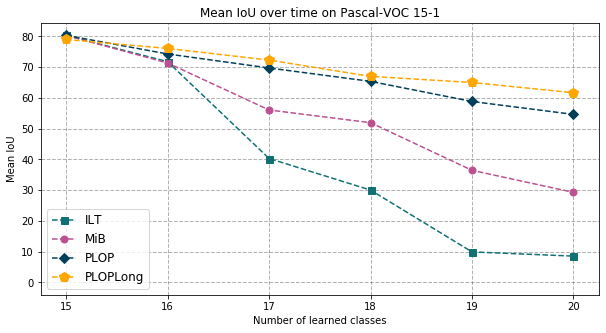
\includegraphics[width=\linewidth]{images/seg/voc_15-1.png}
    \vspace*{-0.3cm}
    \caption{\ac{mIoU} evolution on Pascal-VOC 2012 15-1. While MiB's \ac{mIoU} quickly
        deteriorates, PLOP and PLOPLong's \ac{mIoU} remains high, due to improved resilience to
        catastrophic forgetting.}
    \label{fig:seg_plot_voc_15-1}
\end{figure}

\begin{table*}[t]
    \centering
    \begin{adjustbox}{max width=\textwidth}
        \begin{tabular}{@{}l|cccc||cccc||cccc@{}}
            \toprule
                                                                       & \multicolumn{4}{c}{\textbf{100-50} (2 tasks)} & \multicolumn{4}{c}{\textbf{50-50} (3 tasks)} & \multicolumn{4}{c}{\textbf{100-10} (6 tasks)}                                                                                                                                                                         \\
            \textbf{Method}                                            & 0-100                                         & 101-150                                      & \textit{final}                                & \textit{avg}   & 0-50              & 51-150         & \textit{final}    & \textit{avg}   & 0-100             & 101-150           & \textit{final}    & \textit{avg}   \\
            \midrule
            ILT \scriptsize{\citep{michieli2019ilt}}                   & 18.29                                         & 14.40                                        & 17.00                                         & 29.42          & \tableindent 3.53 & 12.85          & \tableindent 9.70 & 30.12          & \tableindent 0.11 & \tableindent 3.06 & \tableindent 1.09 & 12.56          \\
            MiB \scriptsize{\citep{cermelli2020modelingthebackground}} & 40.52                                         & \textbf{17.17}                               & \textbf{32.79}                                & \textbf{37.31} & 45.57             & \textbf{21.01} & 29.31             & 38.98          & 38.21             & 11.12             & 29.24             & 35.12          \\
            PLOP                                                       & \textbf{41.87}                                & 14.89                                        & \textbf{32.94}                                & \textbf{37.39} & \textbf{48.83}    & \textbf{20.99} & \textbf{30.40}    & \textbf{39.42} & \textbf{40.48}    & \textbf{13.61}    & \textbf{31.59}    & \textbf{36.64} \\
            \bottomrule
        \end{tabular}
    \end{adjustbox}
    \caption{\textbf{ADE20k quantitative experiments} in \ac{mIoU} (\%).}
    \label{tab:seg_ade_sota}
\end{table*}

\begin{table}[t]
    \centering
    \begin{tabular}{@{}l|cccc@{}}
        \toprule
                                                      & \multicolumn{4}{c}{\textbf{VOC 10-1} (11 tasks)}                                                          \\
        \textbf{Method}                               & 0-10                                             & 11-20             & \textit{all}      & \textit{avg}   \\
        \midrule
        ILT \citep{michieli2019ilt}                   & \tableindent 7.15                                & \tableindent 3.67 & \tableindent 5.50 & 25.71          \\
        MiB \citep{cermelli2020modelingthebackground} & 12.25                                            & 13.09             & 12.65             & 42.67          \\
        PLOP                                          & 44.03                                            & 15.51             & 30.45             & 52.32          \\
        PLOPLong                                      & \textbf{61.06}                                   & \textbf{18.56}    & \textbf{40.83}    & \textbf{58.62} \\
        %{\color{red}\ourslong + OR} & \textbf{59.82} & \textbf{22.28} & \textbf{41.95} & \textbf{58.74}\\
        \bottomrule
    \end{tabular}
    \caption{\ac{mIoU} on Pascal-VOC 2012 10-1.}
    \label{tab:seg_voc_hard}
\end{table}

\begin{table}[t]
    \centering
    \begin{tabular}{@{}l|cccc@{}}
        \toprule
                                                      & \multicolumn{4}{c}{\textbf{ADE 100-5} (11 tasks)}                                                                      \\
        \textbf{Method}                               & 0-100                                             & 101-150                    & \textit{all}      & \textit{avg}      \\
        \midrule
        ILT \citep{michieli2019ilt}                   & \tableindent 0.08                                 & \tableindent 1.31          & \tableindent 0.49 & \tableindent 7.83 \\
        MiB \citep{cermelli2020modelingthebackground} & 36.01                                             & \tableindent 5.66          & 25.96             & 32.69             \\
        PLOP                                          & \textbf{39.11}                                    & \tableindent \textbf{7.81} & \textbf{28.75}    & \textbf{35.25}    \\
        % \ourslong & 24.78 & 10.23 & 19.97 & 30.03\\
        \bottomrule
    \end{tabular}
    \caption{\ac{mIoU} on ADE20k 100-5.}
    \label{tab:seg_ade_hard}
\end{table}



\paragraph{Pascal VOC 2012:} \autoref{tab:seg_voc_sota1} shows quantitative experiments on
VOC 19-1, 15-5, and 15-1. Both the proposed PLOP and PLOPLong outperform state-of-the-art
approaches, MiB \citep{cermelli2020modelingthebackground}, SDR \citep{michieli2021sdr}, and GIFS
\citep{cermelli2020fewshotcontinualsegm} on all evaluated settings by a significant margin. For
instance, on 19-1, the forgetting of old classes (1-19) is reduced by 4.39 percentage points (\pp)
while performance on new classes is greatly improved (+13.76 \pp), as compared to the best
performing method so far, MIB \citep{cermelli2020modelingthebackground}. On 15-5, our model is on par
with our re-implementation of MiB, and surpasses the original paper scores
\citep{cermelli2020modelingthebackground} by 1 \pp. On the most challenging 15-1 setting, general
continual models (EWC and LwF-MC) and ILT all have very low \ac{mIoU}. While MiB shows significant
improvements, PLOP still outperforms it by a wide margin. Furthermore, PLOP also significantly
outperform the best performing approach on this setting, GIFS
\cite{cermelli2020fewshotcontinualsegm} (+6.11 \pp). Moreover, \ac{mIoU} for the joint model is
$77.40\%$, thus PLOP narrows the gap between \ac{CSS} and joint learning on every \ac{CSS} scenario. The
average \ac{mIoU} is also improved (+5.78 \pp) compared to GIFS, indicating that each \ac{CSS} step
benefits from the improvements related to our method. This is echoed by
\autoref{fig:seg_plot_voc_15-1}, which shows that while \ac{mIoU} for both ILT and MiB deteriorates
after only a handful of steps, PLOP's \ac{mIoU} remains very high throughout, indicating improved
resilience to catastrophic forgetting and background shift. Last but not least, while PLOP performs
better than PLOPLong on short setups (e.g. 19-1, 15-5), PLOPLong performs better, however, on longer
\ac{CSS} benchmarks such as 15-1 (+2.81 \pp).



\paragraph{Cityscapes:} We also validate our method on Cityscapes in
\autoref{tab:seg_cityscapes_class}. In order to design a setting similar to Pascal-VOC 15-1 (6
tasks), we design the 14-1 setting. Also, we simulate a background class by folding together the
unlabeled classes. Here again, PLOP performs slightly better than MIB (+2.48 \pp on the old classes,
+0.16 \pp on the new ones, +1.15 \pp on average). Moreover, PLOPLong performs significantly better
(+3.59 \pp on the old classes, +2.13 \pp on the new ones, +3.15 \pp on average), indicating better
robustness to both catastrophic forgetting and background shift, especially when considering long
continual learning setups. To more precisely assess this phenomenon, we investigate the performance
of both methods when dealing with longer task learning sequences.

\paragraph{ADE20K:} \autoref{tab:seg_ade_sota} shows experiments on ADE 100-50, 100-10, and
50-50. This dataset is notoriously hard, as the joint model baseline \ac{mIoU} is only 38.90\%. ILT
has poor performance in all three scenarios. PLOP shows comparable performance with MiB on the short
setting 100-50 (only 2 tasks), improves by 1.09 \textit{p.p} on the medium setting 50-50 (3 tasks),
and significantly outperforms MiB with a wider margin of 2.35 \textit{p.p} on the long setting
100-10 (6 tasks). In addition to being better on all settings, PLOP showcased an increased
performance gain on longer \ac{CSS} (e.g. 100-10) scenarios, due to increased robustness to catastrophic
forgetting and background shift.


\paragraph{Longer Continual Trainings:}We argue that \ac{CSS} experiments should push towards
more steps
\citep{wortsman2020supermasks,lomonaco2020ar1,douillard2020podnet,castro2018end_to_end_inc_learn} to
quantify the robustness of approaches w.r.t. catastrophic forgetting and background shift. We
introduce two novel and much more challenging settings with 11 tasks, almost twice as many as the
previous longest setting. We report results for VOC 10-1 in \autoref{tab:seg_voc_hard} (10 classes
followed by 10 times 1 class) and ADE 100-5 in \autoref{tab:seg_ade_hard} (100 classes followed by
10 times 5 classes). The second previous State-of-the-Art method, ILT, has a very low \ac{mIoU}
($<6$ on VOC 10-1 and practically null on ADE 100-5). Furthermore, the gap between PLOP and MiB is
even wider compared with previous benchmarks (e.g. $\times$3.6 \ac{mIoU} on VOC for \ac{mIoU} of
base classes 1-10), which confirms the superiority of PLOP when dealing with long continual
processes. Moreover, in such a case, PLOPlong really shines, bringing significant improvements
(+17.03 \pp on the old classes, +3.05 \pp on the new classes, +10.42 \pp on average) due to
combination of cosine normalization (both on the classifier and Local POD) and its frozen
BatchReNormalization.

\subsubsection{Models Introspection}

We compare several distillation and classification losses on VOC 15-1 to stress the importance of
the components of PLOP and report results in \autoref{tab:seg_ablation_distill_classif}. All
comparisons are evaluated on a val set made with 20\% of the train set, therefore results are
slightly different from the main experiments.

\paragraph{Distillation comparisons:} \autoref{tab:seg_ablation_distillation} compares different
distillation losses when combined with our pseudo-labeling loss. ILT \citep{michieli2019ilt} used
the naive knowledge distillation of \cite{hinton2015knowledge_distillation}. CSC \citep{park2020csc}
constrained spatial and channel correlation of intermediary features. This work bears similarity
with POD and Local POD, but it's much more computationally intensive as it computes pixel-by-pixel
correlation and not as performant. Finally, UNKD introduced in
\cite{cermelli2020modelingthebackground} performs better than the Knowledge Distillation (KD) of
\cite{hinton2015knowledge_distillation}, but not at every step (as indicated by the \textit{avg.}
value), which indicates instability during the training process. POD, proposed in
\cite{douillard2020podnet} (\autoref{chapter:regularization}), improves the results on the old
classes, but not on the new classes (16-20). In fact, due to too much plasticity, POD model likely
overfits and predicts nothing but the new classes, hence a lower \ac{mIoU}.  Finally, Local POD
leads to superior performance (+20 \pp) w.r.t. all metrics, due to its integration of both long and
short-range dependencies. This final row represents our full PLOP strategy.


\paragraph{Classification comparisons:} \autoref{tab:seg_ablation_classif} compares different
classification losses when combined with our Local POD distillation loss. Cross-Entropy (CE)
variants perform poorly, especially on new classes. UNCE, introduced in
\citep{cermelli2020modelingthebackground}, improves by merging the background with old classes,
however, it still struggles to correctly model the new classes, whereas our pseudo-labeling
propagates more finely information of the old classes, while learning to predict the new ones,
dramatically enhancing the performance in both cases. This penultimate row represents our full PLOP
strategy. Also notice that the performance for pseudo-labeling is very close to
\textit{(Oracle) Pseudo-good} (where the incorrect pseudo-labels are removed), which may constitute a
performance ceiling of our uncertainty measure. A comparison between these two results illustrates
the relevance of our entropy-based uncertainty estimate. \textit{(Oracle) Pseudo-corrected} is
similar to the previous oracle but instead fix the incorrect pseudo-labels; note that not all labels
are present as some pixels were not even pseudo-labelized due to their high uncertainty. Finally,
\textit{(Oracle) CE + all labels} has access to all labels of previous and current classes
$\mcC^{1:t}$.

\subsubsection{Robustness to class ordering}

Continual learning methods may be prone to instability. It has already been shown in related
contexts \citep{kim2019medic} that class ordering can have a large impact on performance.
Unfortunately, in real-world settings, the optimal class order can never be known beforehand: thus,
the performance of an ideal \ac{CSS} method should be as invariant to class order as possible. In all
experiments done so far, this class order has been kept constant, as defined
by \cite{cermelli2020modelingthebackground}. We report results in \autoref{fig:seg_order_voc_15-1}
as boxplots obtained by applying 20 random permutations of the class order on VOC 15-1. We report in
\autoref{fig:seg_order_voc_15-1} (from left to right) the \ac{mIoU} for the old, new classes, all
classes, and average over \ac{CSS} steps. In all cases, PLOP surpasses MiB in terms of avg \ac{mIoU}.
Furthermore, the standard deviation (e.g. 10\% vs 5\% on \textit{all}) is always significantly
lower, showing the excellent stability of PLOP compared with existing approaches. Moreover,
PLOPLong, while having more variance on the new classes, performs better overall as compared to
PLOP, not to mention MiB. This is due to the fact that PLOPLong, due to improved distillation loss
(at prediction and Local POD levels) and batch re-normalization that allows to better retain
information of the old classes, which again is more conspicuous on longer \ac{CSS} scenarios.

\begin{table}
    \centering
    \caption{Comparison studies on Pascal-VOC 2012 15-1 on a validation subset of 20\% of the training set.}
    %\vspace*{-0.3cm}
    \label{tab:ablation_distill_classif}
    \begin{subtable}{0.5\textwidth}
        \centering
        \caption{Pseudo loss (\autoref{eq:pseudo_loss}) with different distillation losses.}
        %\vspace*{-0.2cm}
        \label{tab:ablation_distillation}
        \begin{tabular}{@{}l|cccc@{}}
            \toprule
            Distillation loss                       & 0-15           & 16-20             & \textit{all}   & \textit{avg}   \\
            \midrule
            %ILT \cite{michieli2019ilt}'s distill & 19.91 & \tableindent 5.49 & 16.48 & 49.43\\
            %CSC \cite{park2020csc} & 25.49 & \tableindent 4.72 & 20.48 & 44.97\\
            Knowledge Distillation                  & 29.72          & \tableindent 4.42 & 23.69          & 49.18          \\
            UNKD                                    & 34.85          & \tableindent 5.26 & 27.80          & 46.39          \\
            POD                                     & 43.94          & \tableindent 4.82 & 34.62          & 53.35          \\
            Local POD (\autoref{eq:local_pod_loss}) & \textbf{63.06} & \textbf{17.92}    & \textbf{52.31} & \textbf{65.71} \\
            \bottomrule
        \end{tabular}
    \end{subtable}
    \hfill
    \vspace{0.5cm}
    \begin{subtable}{0.5\textwidth}
        \centering
        \caption{Local POD loss (\autoref{eq:local_pod_loss}) with different classification losses.}
        %\vspace*{-0.2cm}
        \label{tab:ablation_classif}
        \begin{tabular}{@{}l|cccc@{}}
            \toprule
            Classification loss               & 0-15           & 16-20             & \textit{all}   & \textit{avg}   \\
            \midrule
            CE only on new                    & 12.95          & \tableindent 2.54 & 10.47          & 47.02          \\
            CE                                & 33.80          & \tableindent 4.67 & 26.87          & 50.79          \\
            UNCE                              & 48.46          & \tableindent 4.82 & 38.62          & 53.19          \\
            Pseudo (\autoref{eq:pseudo_loss}) & \textbf{63.06} & \textbf{17.92}    & \textbf{52.31} & \textbf{65.71} \\
            \midrule
            \textit{\small{Pseudo-Oracle}}    & \textit{63.69} & \textit{23.35}    & \textit{54.09} & \textit{66.05} \\
            %\textit{\small{Pseudo + corrected}} & \textit{66.88} & \textit{16.88} & \textit{54.98} & \textit{66.50}\\
            %\textit{\small{CE + all labels}}  & \textit{71.45} & \textit{10.78} & \textit{57.00} & \textit{67.04}\\
            \bottomrule
        \end{tabular}
    \end{subtable}
\end{table}






\begin{figure}
    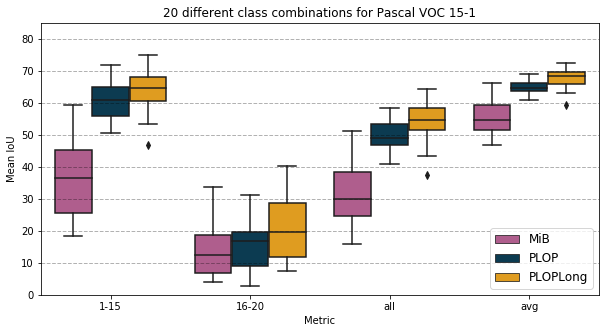
\includegraphics[width=\linewidth]{images/seg/order_voc_15-1.png}
    \vspace*{-0.3cm}
    \caption{Boxplots of the \ac{mIoU} of initial classes (1-15), new (16-20), all, and average for
        20 random class orderings. PLOP is significantly better and more stable than MiB. PLOPLong
        further improves upon PLOP by better retaining old class information.}
    \label{fig:seg_order_voc_15-1}
\end{figure}


\subsection{Object Rehearsal experiments}

\subsubsection{Quantitative Evaluations}

\begin{table*}[t]
    \centering
    \caption{Comparison of rehearsal-based methods on Pascal-VOC 2012 15-1 overlap in Mean IoU (\%). We only consider the time overhead spent after the first task whose computation overhead is similar for all methods.}
    \vspace*{-0.3cm}
    \label{tab:voc_rehearsal_learning}
    \begin{tabular}{@{}l|ccc|cccc@{}}
        \toprule
                                                                & \multicolumn{7}{c}{\textbf{15-1} (6 tasks)}                                                                                                                                              \\
        \textbf{Method}                                         & \textbf{Rehearsal}                          & \textbf{Memory} (Mb) $\downarrow$ & \textbf{Time} (Hours) $\downarrow$ & 0-15           & 16-20          & \textit{all}   & \textit{avg}   \\
        \midrule
        PLOP                                                    & ---                                         & 0                                 & 1.8                                & 65.12          & 21.11          & 54.64          & 67.21          \\
        PLOPLong                                                & ---                                         & 0                                 & 1.8                                & 72.00          & 26.66          & 61.20          & 70.02          \\
        %HRHF \cite{huang2021halfrealhalffake} & DeepInversion & 0 & 5.9 & 72.40 & 39.60 & 64.60 & \\
        \hdashline
        Yu et al.\cite{yu2020continualsegmentationselftraining} & Unlabeled COCO                              & 20,000                            & 7.0                                & 71.40          & 40.00          & 63.60          &                \\
        PLOP                                                    & Unlabeled COCO                              & 20,000                            & 1.4                                & 72.57          & 45.08          & 66.03          & 71.85          \\
        PLOP                                                    & Unlabeled VOC                               & 2,000                             & 1.4                                & 75.32          & 52.59          & 69.91          & 75.21          \\
        %PLOP & Partial VOC & 2,000 & \tbd & 74.91 & 54.55 & 70.06 & 75.41 \\
        %PLOPv2 & Partial VOC & 2,000  & \tbd & 76.87 & 56.07 & 71.92 & 74.88\\
        \hdashline
        PLOPLong                                                & Partial VOC                                 & 2.2                               & 2.6                                & 74.14          & 38.87          & 65.74          & 72.02          \\
        PLOPLong                                                & Partial VOC                                 & 22                                & 2.6                                & \textbf{74.18} & 43.22          & 66.81          & \textbf{72.48} \\
        PLOPLong                                                & Object VOC                                  & 0.26                              & 2.7                                & 73.32          & 42.86          & 66.07          & 72.21          \\
        PLOPLong                                                & Object VOC                                  & 2.6                               & 2.7                                & 73.79          & \textbf{45.78} & \textbf{67.12} & \textbf{72.42} \\
        \midrule
        Joint model                                             & ---                                         & ---                               & ---                                & 79.10          & 72.60          & 77.40          & ---            \\
        \bottomrule
    \end{tabular}
\end{table*}


\paragraph{Pascal-VOC 15-1:} We now allow \ac{CSS} models to store information from the previous
steps and classes: in such a case, the overall model efficiency can be understood as to what extent
it allows to find good trade-off between its accuracy (as measured by the aforementionned standard
metrics) and the memory footprint of the stored images or objects. Methods such as HRHF
\citep{huang2021halfrealhalffake} can not easily be understood in these terms as they do not store
data, strictly speaking, but rather use deep inversion \citep{yin20deepinversion} techniques to
generate synthetic data, which comes at a high time requirement: thus, we exclude this method from
our comparisons. We first consider the challenging Pascal-VOC 15-1 setting in
\autoref{tab:seg_voc_rehearsal_learning}. We use PLOP and PLOPLong as baselines with 0 memory
overhead, as both models only use data from the current task. Moreover, we compare with
\cite{yu2020continualsegmentationselftraining}, where an unlabeled external dataset such as COCO
\citep{lin2014mscocodataset} is used through pseudo-labelling to improve performance on Pascal-VOC,
as both datasets present significant overlap in terms of classes and domains. We reimplemented their
method and also considered PLOP in this configuration. Using the external COCO provide PLOP an
important gain of \ac{mIoU} for both old classes (+7 \pp) and new classes (+24
\pp). Furthermore, PLOP with COCO is significantly more performant than Yu et al. model
(+5.43 \pp) despite the latter was designed explicitly to use such unlabeled external
dataset. Notice also how PLOPLong, without any kind of rehearsal, remains equivalent to
\cite{yu2020continualsegmentationselftraining} in terms of \ac{mIoU} on 0-15 (72.00\% vs 71.40\%),
despite the latter using a large pool of data (+20Go). Perhaps counter-intuitively the gain is
located on the new classes (26.66\% vs 40.00\%) as the rehearsal effect has a regularizing effect
leading to less over-predicting of the recent classes. A drawback of using COCO is that the visual
domain is not exactly the same as VOC, therefore we also considered using PLOP with a rehearsal of
the unlabeled VOC. Without surprise, it results in a much better overall performance (+3.88
\pp compared to using COCO). Another setup that we consider is the image rehearsal
paradigm, where, at each step, we keep a number of (randomly selected) images along with their
segmentation map. These segmentation maps are however incomplete, due to the nature of the \ac{CSS}
problem (see \autoref{sec:seg_object_rehearsal}): hence, we refer to this setting as partial VOC. We
consider two amounts of images to keep: 10 images per class (22 Mb) and 1 image per class (2.2 Mb).
PLOPLong largely benefits from this rehearsal, most notably on new classes (16-20) with a gain up to
16.56 \pp. Finally, we compare our novel Object Rehearsal denoted by ``\textit{object
    VOC}'' where we store either one object per class (0.26 Mb) or 10 objects per class (2.6 Mb). As
shown on \autoref{tab:seg_voc_rehearsal_learning}, The proposed object rehearsal, in addition to
being significantly more memory efficient than whole image rehearsal (8.5$\times$ less space used),
is equivalent or better in terms of \ac{mIoU} especially for new classes (2.56 \pp). The
ensemble of our experiments proves that rehearsal, when the partial or missing labeling is carefully
handled, can provide important performance gain. Furthermore, our novel object rehearsal manages to
strike the best trade-off with a minimal memory overhead without impacting its performance.

\begin{comment}
\begin{figure}
    \centering
    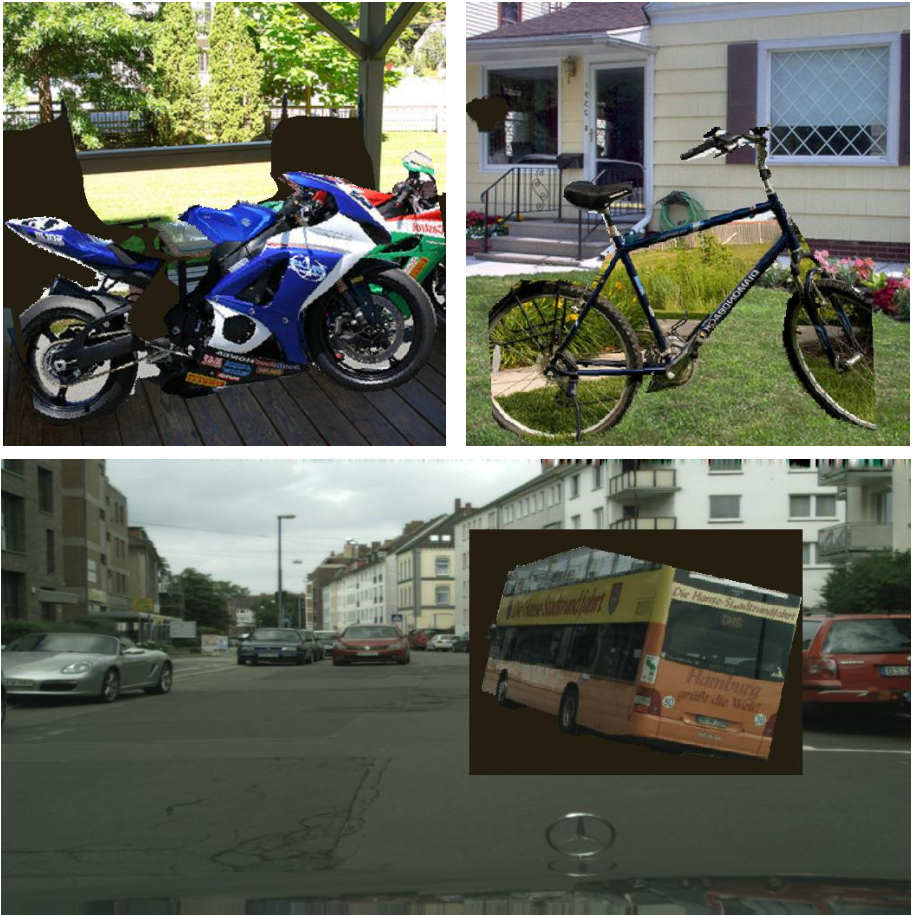
\includegraphics[width=0.5\linewidth]{images/seg/object_pasting.pdf}
    \caption{Pasted object for rehearsal in three images. Top row shows the pasting of a
        \texttt{motorbike} and a \texttt{bicycle} in Pascal-VOC, and bottom row shows the pasting of
        a \texttt{bus} in Cityscapes.}
    \label{fig:seg_object_pasting}
\end{figure}
\end{comment}

\paragraph{Cityscapes:} We propose more experiments with Object Rehearsal in
\autoref{tab:seg_cityscapes_rehearsal} where we apply our model on Cityscapes 14-1. For the rehearsal,
we sample either 10 images or object per class. Cityscapes images are particularly large (even
resized to $512 \times 1024$)  and "empty" (most of it is road and sky). Consequently, the memory
overhead is extremely important compared object rehearsal (117 vs 0.8). We show that both our novel
image and object rehearsal improve performance of the already competitive PLOPLong, and with object
rehearsal providing the large gain (+9 \pp in \textit{all}).

t\begin{table}[t]
    \centering
    \begin{adjustbox}{max width=\textwidth}
        \begin{tabular}{@{}l|cc|cccc@{}}
            \toprule
                                                                       & \multicolumn{6}{c}{\textbf{14-1} (6 tasks)}                                                                                       \\
            \textbf{Method}                                            & \textbf{Rehearsal}                          & \textbf{Memory} & 1-14           & 15-19          & \textit{final} & \textit{avg}   \\
            \midrule
            MiB \scriptsize{\citep{cermelli2020modelingthebackground}} & ---                                         & 0               & 55.11          & 12.91          & 44.56          & 49.76          \\
            PLOP                                                       & ---                                         & 0               & 56.59          & 13.07          & 45.71          & 51.28          \\
            PLOPLong                                                   & ---                                         & 0               & 58.60          & 15.04          & 47.71          & 54.31          \\
            PLOPLong                                                   & Partial                                     & 117.0           & \textbf{58.93} & 19.55          & 49.09          & \textbf{55.74} \\
            PLOPLong                                                   & Object                                      & 0.8             & 57.82          & \textbf{23.13} & \textbf{49.15} & 54.80          \\
            \bottomrule
        \end{tabular}
    \end{adjustbox}
    \caption{\textbf{Cityscapes quantitative experiments with rehearsal} on Cityscapes 14-1 overlap in \ac{mIoU} (\%).}
    \label{tab:seg_cityscapes_rehearsal}
\end{table}

\begin{table}[t]
    \centering
    \begin{tabular}{@{}llc|c|cc|r@{}}
        \toprule
                                &                 &                &                                & \multicolumn{2}{c}{\textbf{15-1} (6 tasks)}                         \\
        \textbf{Type}           & \textbf{Mixing} & \textbf{Erase} & \textbf{Memory} $\downarrow$   & \textit{final}                              & \textit{avg}   &      \\
        \midrule
        \multirow{2}{*}{Image}  & Mixup           & ---            & \multirow{2}{*}{22.20}         & 61.77                                       & 69.88          & I    \\
                                & \,\,\,\,\,---   & ---            &                                & 66.81                                       & \textbf{72.48} & II   \\
        \hline
        \multirow{3}{*}{Patch}  & Pasting         & All            & \multirow{3}{*}{4.50}          & 55.45                                       & 66.35          & III  \\
                                & Pasting         & ---            &                                & 63.41                                       & 70.75          & IV   \\
                                & Pasting         & Foreground     &                                & 66.28                                       & 71.66          & V    \\
        \hline
        \multirow{5}{*}{Object} & Mixup           & ---            & \multirow{5}{*}{\textbf{2.60}} & 63.25                                       & 70.91          & VI   \\
                                & Mixup           & Foreground     &                                & 64.45                                       & 71.65          & VII  \\
                                & Pasting         & All            &                                & 52.26                                       & 65.97          & VIII \\
                                & Pasting         & ---            &                                & 63.12                                       & 70.52          & IX   \\
                                & Pasting         & Foreground     &                                & \textbf{67.12}                              & \textbf{72.42} & X    \\
        \bottomrule
    \end{tabular}
    \caption{\textbf{Rehearsal alternatives} on Pascal-VOC 2012 in \ac{mIoU} (\%). Object/Patch-based methods
        with 10 objects/patches per class, and Image-based with 10 images per class. All
        experiments done with PLOPLong.}
    \label{tab:seg_rehearsal_alternative}
\end{table}


\begin{figure}
    \centering
    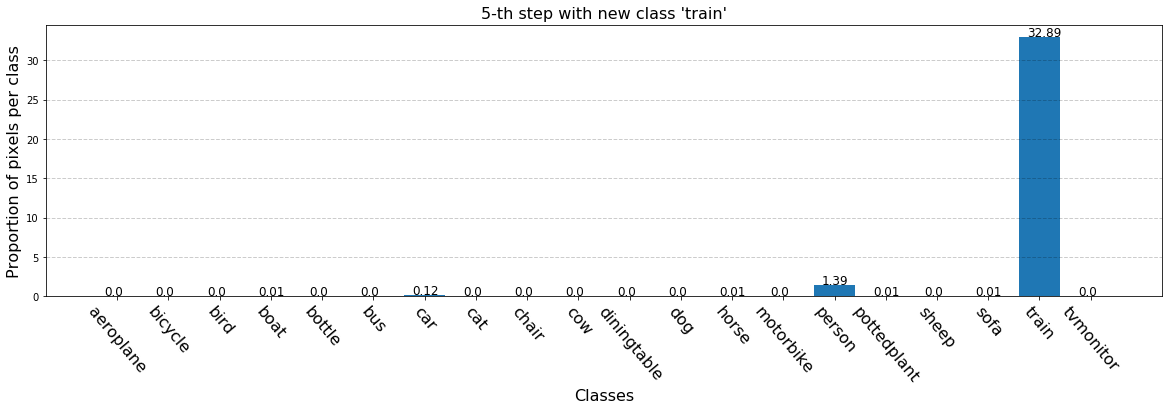
\includegraphics[width=\linewidth]{images/seg/distribution_5step_voc.png}
    \vspace*{-0.3cm}
    \caption{Distribution of the pixel per class during the $5^{\text{th}}$ step of Pascal-VOC
        15-1.}
    \label{fig:seg_distribution_voc_5th}
\end{figure}

\begin{figure*}
    \centering
    \includegraphics[width=\linewidth]{images/seg/visualization2.pdf}
    \caption{Visualization of the predictions of MiB, PLOP, PLOPLong, and PLOPLong with Object
        Rehearsal on three test images at the $6^\text{th}$ and final step on VOC 15-1 scenario. The
        first image contains \texttt{car}, \texttt{cow}, and \texttt{person}; the second
        \texttt{plane} and \texttt{bus}, and the third \texttt{bicycle} and \texttt{person}. While
        MiB doesn't manage to predict the correct classes, and tends to overpredict the most recent
        ones (e.g. \texttt{train} in light green). PLOP mostly grasp the correct classes, though
        sometimes with imprecision. PLOPLong and \textit{a fortiori} PLOPLong + Object rehearsal
        captures all existing classes, with the latter predicting almost perfect segmentation masks,
        compared to the ground-truth.}
    \label{fig:seg_visualization}
\end{figure*}

\subsubsection{Object Rehearsal Introspection}

\autoref{tab:seg_rehearsal_alternative} draws a comparison between several rehearsal alternatives in
\ac{CSS}. We split methods according to three criterions: ``\textit{type}'' denotes whether we store a
whole image, an object, or a patch For both object and patch, we only rehearse a small amount of the
images: in object, only the pixel's objects are used while for patch, we use the pixel's object and
the close surrounding pixels that contain background information. We insert the reheasal data
according to ``\textit{mixing}'', either by pasting (see \autoref{sec:seg_object_rehearsal}), by
mixing pixels according to mixup \citep{hingyi2018mixup} rule, or in the case of image rehearsal no
mixing is done. Finally we consider two erasing methods: either all pixels are erased
(\textit{All}), or only pixels belonging to non-background classes are erased (\textit{Foreground}).
Note that, for the latter method, it includes classes detected via pseudo-labeling. For all methods,
we randomly select 10 images/patches/objects per class for rehearsal. Without surprise, Patch
(III-V) and Object-based (VI-X) rehearsal are more data-efficient than images (I and II) (4.50 and
2.60 vs 22.20 Mb). Mixing the rehearsed data with mixup (VI and VII) is less efficient than direct
pasting (III, IV, and VIII-X) because segmentation, contrary to classification, requires sharp
boundaries \citep{chen2020semeda}. We considered rehearsing each patch/object without mixing, but
because their shape may variate no batching is possible which would be much slower. Therefore, we
investigate mixing patches/objects while erasing all others pixels (III and VIII). This doesn't
work, which is probably linked to the altered statistics of the batch normalization. On the other
hand, we found that a selective erasing that remove foreground objects (V, VII, and X) while keeping
the background of the destination image proved to be very effective (63.12\% to 67.12\% \textit{all}
\ac{mIoU} for object). This confirmed our intuition that pasting in segmentation is a delicate
operation that may lead to confusion in the network, particularly on object boundaries. The erased
pixels are replaced by gray pixels. We considered more complicated approaches such as in-painting
\citep{fang2019instaboost} or textures filling \citep{mallikarjuna2006kth-tips}, but were slightly
less effective than our simpler solution. Overall, through careful design, we manage to get the best
performance using our novel object rehearsal which was also the most memory-efficient.

\begin{figure}
    \centering
    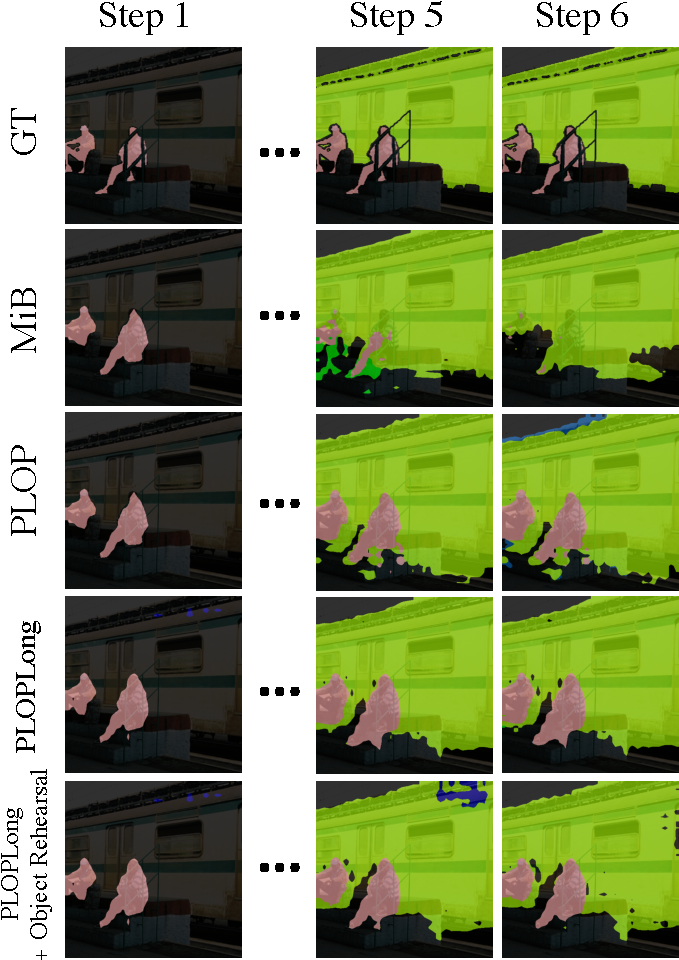
\includegraphics[width=\linewidth]{images/seg/visualization_gt_shift2.pdf}
    \caption{Visualization of the predictions of MiB, PLOP, PLOPLong, and PLOPLong with Object
        Rehearsal across time in VOC 15-1 on a test set image. At steps 1-4 only class
        \texttt{person} has been seen. At step 5, the class \texttt{train} is introduced, causing
        dramatic background shift. While MiB overfits on the new class and forget the old class,
        PLOP is able to predict both classes correctly. PLOPLong and PLOPLong + Object Rehearsal
        further refine the predicted masks, resulting in much sharper boundaries.}
    \label{fig:seg_visualization_gt_shift}
\end{figure}

\paragraph{Rehearsal alleviates pseudo-labeling's limitation:} All previous methods, PLOP
and PLOPLong included, didn't consider rehearsal-learning. While popular in image classification, it
has fewly been explored for continual segmentation. An attentive reader may wonder if rehearsal
learning can have benefit given the fact that our pseudo-labeling can uncover ``hidden'' old classes
in the images. Even a perfect pseudo-labeling (considered in \autoref{tab:seg_ablation_classif}) may
fail in some particular data situation where the class distribution of a step is almost dirac. We
show in \autoref{fig:seg_distribution_voc_5th} the distribution of pixels per class at the
$5^{\text{th}}$ step of Pascal-VOC 15-1. The new class to learn, \texttt{train}, is abundant but
also almost alone but the class \texttt{person}. In this case, no amount of pseudo-labeling can
uncover previous classes like \texttt{bicycle} or \texttt{cat}. Our proposed rehearsal learning is
complementary to our pseudo-labeling loss where the former can reduce the weakness for the latter in
some cases.

\subsection{Visualization}

\autoref{fig:seg_visualization} shows the predictions at the $6^\text{th}$ and final step of VOC
15-1 for four different models: MiB, PLOP, PLOPLong, and PLOPLong with Object Rehearsal. MiB
struggles to even find the correct classes: in the first image the \texttt{car} is predicted as
\texttt{train}, in the second the \texttt{plane} as \texttt{train}, and in the third no classes are
detected. On the other hand, PLOP always manages to pick up the present classes, although sometimes
with imperfection. PLOPLong further refines results, and the addition of Object Rehearsal produces a
sharp and near perfect masks compared to the ground-truths (GTs). We showcased the harmful effect of
background shift in \autoref{fig:seg_visualization_gt_shift} where the class \texttt{person} is
learned at $1^\text{st}$ step and the class \texttt{train} at $5^\text{th}$ step. MiB completly
forgets the former class and overpredict the latter. The background shift is efficiently mitigated
with pseudo-labeling as showed by the third row of PLOP. Our efficient proposition of object
rehearsal allows further refinement of the predicted masks resulting in sharper boundaries.

\section{Conclusion}
\label{sec:seg_conclusion}

Continual Semantic Segmentation (\ac{CSS}) is an emerging but challenging computer vision domain. In this
paper, we highlighted two major issues in \ac{CSS}: catastrophic forgetting and background shift. To deal
with the former, we proposed Local POD, a multi-scale distillation scheme that preserves both long
and short-range spatial statistics between pixels. This lead to an effective balance between
rigidity and plasticity for \ac{CSS}, which in turns alleviate catastrophic forgetting. We then tackled
background shift with an efficient uncertainty-based pseudo-labeling loss. It completes the
partially-labeled segmentation maps, allowing the network to efficiently retain previously learned
knowledge. Afterwards, We showed that carefully designed structural changes to the model could
improve performance on long \ac{CSS} scenarios, namely a cosine normalization adaptation of the
classifier and Local POD followed by a modified batch normalization. Finally, we proposed to
introduce rehearsal learning to \ac{CSS}, one based on partially-labeled whole image rehearsal, and the
other --much more memory-efficient-- consisting in object rehearsal. The latter further refining our
already effective model performance and allowing real world application of \ac{CSS} with a stringent
memory constraint. We evaluated the proposed PLOPLong, with or without object rehearsal, on three
datasets and over twelve different benchmarks. In each, we showed that our model performs
significantly better than all existing baselines. Finally, we qualitatively validate our model
through extensive ablations in order to better understand the performance gain.
